\documentclass[1p]{elsarticle_modified}
%\bibliographystyle{elsarticle-num}

%\usepackage[colorlinks]{hyperref}
%\usepackage{abbrmath_seonhwa} %\Abb, \Ascr, \Acal ,\Abf, \Afrak
\usepackage{amsfonts}
\usepackage{amssymb}
\usepackage{amsmath}
\usepackage{amsthm}
\usepackage{scalefnt}
\usepackage{amsbsy}
\usepackage{kotex}
\usepackage{caption}
\usepackage{subfig}
\usepackage{color}
\usepackage{graphicx}
\usepackage{xcolor} %% white, black, red, green, blue, cyan, magenta, yellow
\usepackage{float}
\usepackage{setspace}
\usepackage{hyperref}

\usepackage{tikz}
\usetikzlibrary{arrows}

\usepackage{multirow}
\usepackage{array} % fixed length table
\usepackage{hhline}

%%%%%%%%%%%%%%%%%%%%%
\makeatletter
\renewcommand*\env@matrix[1][\arraystretch]{%
	\edef\arraystretch{#1}%
	\hskip -\arraycolsep
	\let\@ifnextchar\new@ifnextchar
	\array{*\c@MaxMatrixCols c}}
\makeatother %https://tex.stackexchange.com/questions/14071/how-can-i-increase-the-line-spacing-in-a-matrix
%%%%%%%%%%%%%%%

\usepackage[normalem]{ulem}

\newcommand{\msout}[1]{\ifmmode\text{\sout{\ensuremath{#1}}}\else\sout{#1}\fi}
%SOURCE: \msout is \stkout macro in https://tex.stackexchange.com/questions/20609/strikeout-in-math-mode

\newcommand{\cancel}[1]{
	\ifmmode
	{\color{red}\msout{#1}}
	\else
	{\color{red}\sout{#1}}
	\fi
}

\newcommand{\add}[1]{
	{\color{blue}\uwave{#1}}
}

\newcommand{\replace}[2]{
	\ifmmode
	{\color{red}\msout{#1}}{\color{blue}\uwave{#2}}
	\else
	{\color{red}\sout{#1}}{\color{blue}\uwave{#2}}
	\fi
}

\newcommand{\Sol}{\mathcal{S}} %segment
\newcommand{\D}{D} %diagram
\newcommand{\A}{\mathcal{A}} %arc


%%%%%%%%%%%%%%%%%%%%%%%%%%%%%5 test

\def\sl{\operatorname{\textup{SL}}(2,\Cbb)}
\def\psl{\operatorname{\textup{PSL}}(2,\Cbb)}
\def\quan{\mkern 1mu \triangleright \mkern 1mu}

\theoremstyle{definition}
\newtheorem{thm}{Theorem}[section]
\newtheorem{prop}[thm]{Proposition}
\newtheorem{lem}[thm]{Lemma}
\newtheorem{ques}[thm]{Question}
\newtheorem{cor}[thm]{Corollary}
\newtheorem{defn}[thm]{Definition}
\newtheorem{exam}[thm]{Example}
\newtheorem{rmk}[thm]{Remark}
\newtheorem{alg}[thm]{Algorithm}

\newcommand{\I}{\sqrt{-1}}
\begin{document}

%\begin{frontmatter}
%
%\title{Boundary parabolic representations of knots up to 8 crossings}
%
%%% Group authors per affiliation:
%\author{Yunhi Cho} 
%\address{Department of Mathematics, University of Seoul, Seoul, Korea}
%\ead{yhcho@uos.ac.kr}
%
%
%\author{Seonhwa Kim} %\fnref{s_kim}}
%\address{Center for Geometry and Physics, Institute for Basic Science, Pohang, 37673, Korea}
%\ead{ryeona17@ibs.re.kr}
%
%\author{Hyuk Kim}
%\address{Department of Mathematical Sciences, Seoul National University, Seoul 08826, Korea}
%\ead{hyukkim@snu.ac.kr}
%
%\author{Seokbeom Yoon}
%\address{Department of Mathematical Sciences, Seoul National University, Seoul, 08826,  Korea}
%\ead{sbyoon15@snu.ac.kr}
%
%\begin{abstract}
%We find all boundary parabolic representation of knots up to 8 crossings.
%
%\end{abstract}
%\begin{keyword}
%    \MSC[2010] 57M25 
%\end{keyword}
%
%\end{frontmatter}

%\linenumbers
%\tableofcontents
%
\newcommand\colored[1]{\textcolor{white}{\rule[-0.35ex]{0.8em}{1.4ex}}\kern-0.8em\color{red} #1}%
%\newcommand\colored[1]{\textcolor{white}{ #1}\kern-2.17ex	\textcolor{white}{ #1}\kern-1.81ex	\textcolor{white}{ #1}\kern-2.15ex\color{red}#1	}

{\Large $\underline{11a_{297}~(K11a_{297})}$}

\setlength{\tabcolsep}{10pt}
\renewcommand{\arraystretch}{1.6}
\vspace{1cm}\begin{tabular}{m{100pt}>{\centering\arraybackslash}m{274pt}}
\multirow{5}{120pt}{
	\centering
	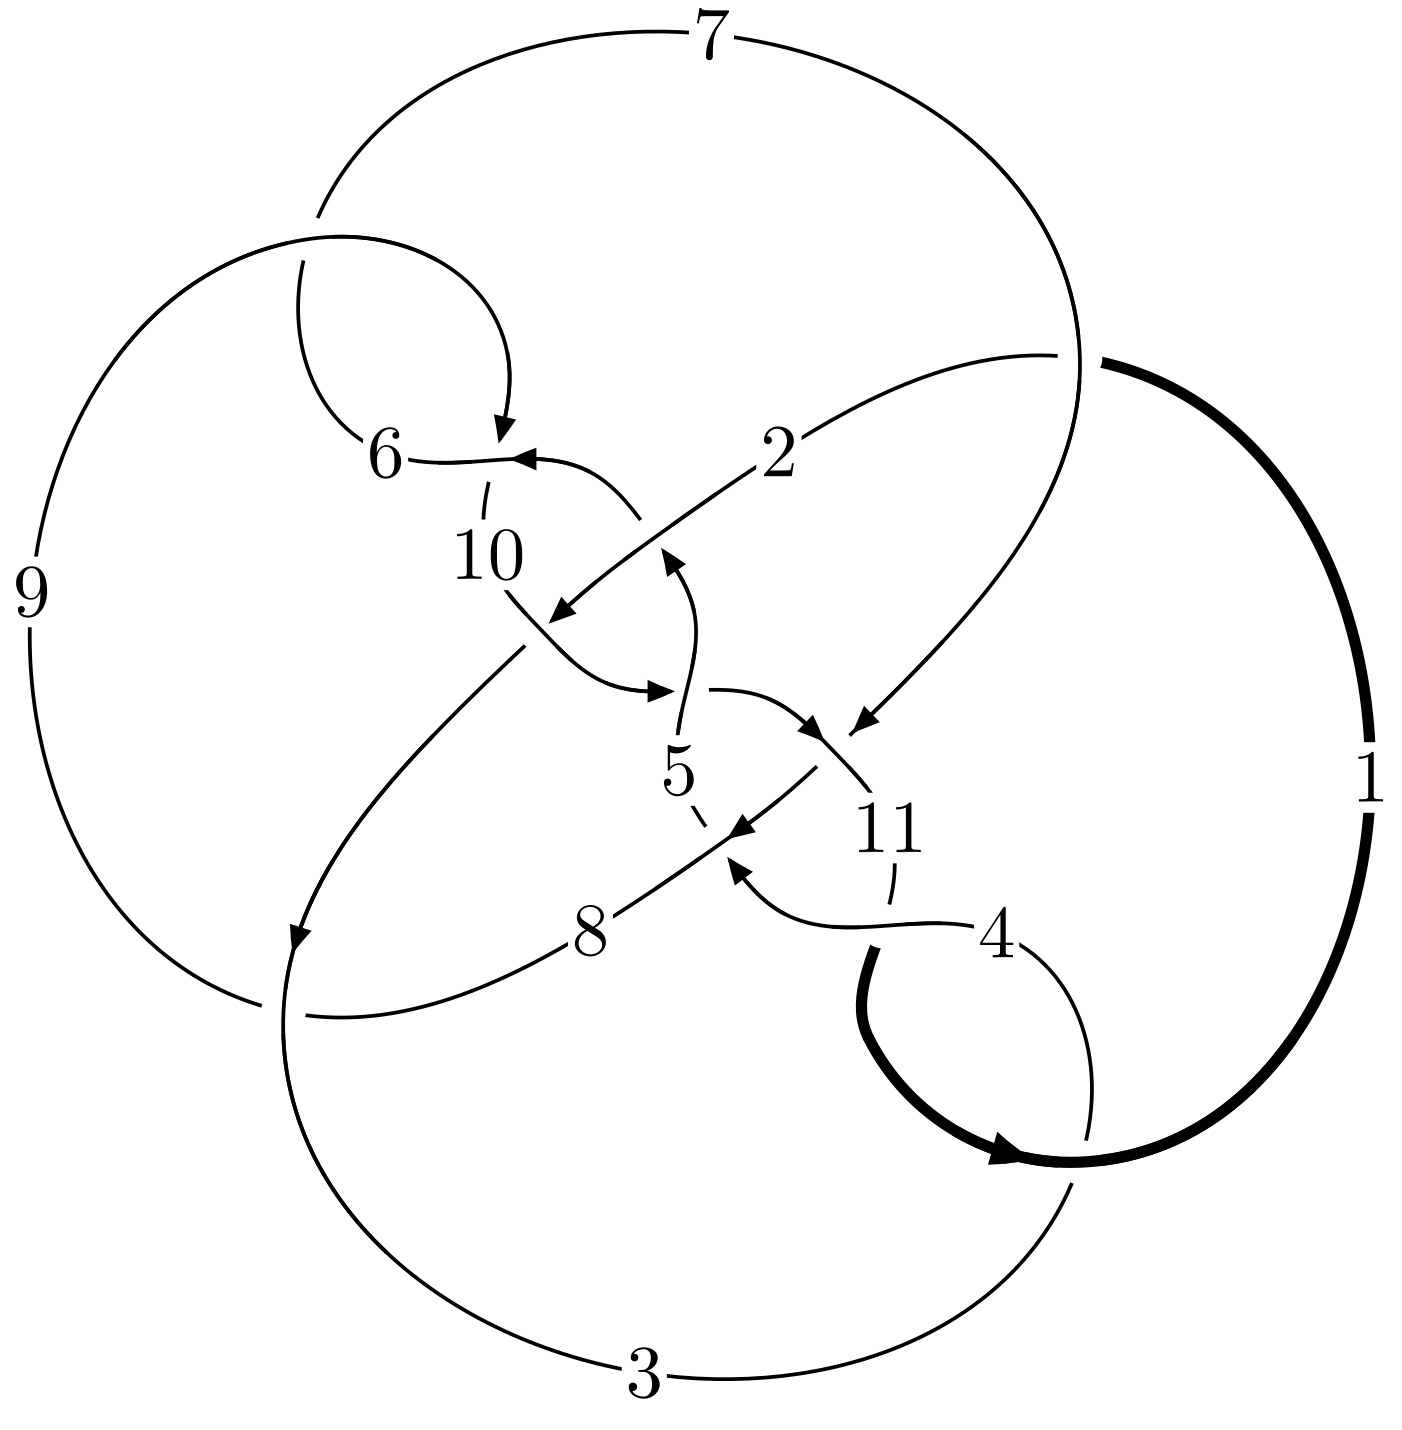
\includegraphics[width=112pt]{../../../GIT/diagram.site/Diagrams/png/546_11a_297.png}\\
\ \ \ A knot diagram\footnotemark}&
\allowdisplaybreaks
\textbf{Linearized knot diagam} \\
\cline{2-2}
 &
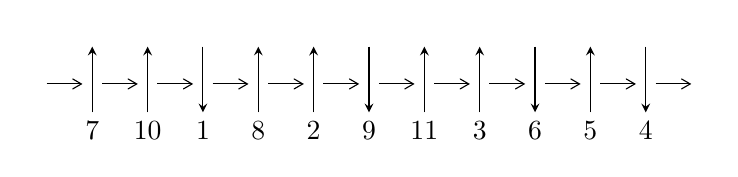
\begin{tikzpicture}[x=20pt, y=17pt]
	% nodes
	\node (C0) at (0, 0) {};
	\node (C1) at (1, 0) {};
	\node (C1U) at (1, +1) {};
	\node (C1D) at (1, -1) {7};

	\node (C2) at (2, 0) {};
	\node (C2U) at (2, +1) {};
	\node (C2D) at (2, -1) {10};

	\node (C3) at (3, 0) {};
	\node (C3U) at (3, +1) {};
	\node (C3D) at (3, -1) {1};

	\node (C4) at (4, 0) {};
	\node (C4U) at (4, +1) {};
	\node (C4D) at (4, -1) {8};

	\node (C5) at (5, 0) {};
	\node (C5U) at (5, +1) {};
	\node (C5D) at (5, -1) {2};

	\node (C6) at (6, 0) {};
	\node (C6U) at (6, +1) {};
	\node (C6D) at (6, -1) {9};

	\node (C7) at (7, 0) {};
	\node (C7U) at (7, +1) {};
	\node (C7D) at (7, -1) {11};

	\node (C8) at (8, 0) {};
	\node (C8U) at (8, +1) {};
	\node (C8D) at (8, -1) {3};

	\node (C9) at (9, 0) {};
	\node (C9U) at (9, +1) {};
	\node (C9D) at (9, -1) {6};

	\node (C10) at (10, 0) {};
	\node (C10U) at (10, +1) {};
	\node (C10D) at (10, -1) {5};

	\node (C11) at (11, 0) {};
	\node (C11U) at (11, +1) {};
	\node (C11D) at (11, -1) {4};
	\node (C12) at (12, 0) {};

	% arrows
	\draw[->,>={angle 60}]
	(C0) edge (C1) (C1) edge (C2) (C2) edge (C3) (C3) edge (C4) (C4) edge (C5) (C5) edge (C6) (C6) edge (C7) (C7) edge (C8) (C8) edge (C9) (C9) edge (C10) (C10) edge (C11) (C11) edge (C12) ;	\draw[->,>=stealth]
	(C1D) edge (C1U) (C2D) edge (C2U) (C3U) edge (C3D) (C4D) edge (C4U) (C5D) edge (C5U) (C6U) edge (C6D) (C7D) edge (C7U) (C8D) edge (C8U) (C9U) edge (C9D) (C10D) edge (C10U) (C11U) edge (C11D) ;
	\end{tikzpicture} \\
\hhline{~~} \\& 
\textbf{Solving Sequence} \\ \cline{2-2} 
 &
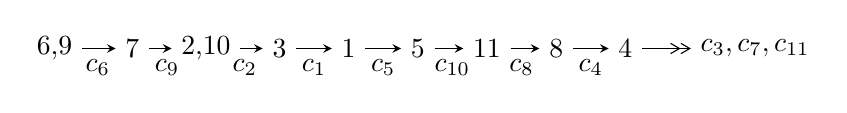
\begin{tikzpicture}[x=25pt, y=7pt]
	% node
	\node (A0) at (-1/8, 0) {6,9};
	\node (A1) at (1, 0) {7};
	\node (A2) at (33/16, 0) {2,10};
	\node (A3) at (25/8, 0) {3};
	\node (A4) at (33/8, 0) {1};
	\node (A5) at (41/8, 0) {5};
	\node (A6) at (49/8, 0) {11};
	\node (A7) at (57/8, 0) {8};
	\node (A8) at (65/8, 0) {4};
	\node (C1) at (1/2, -1) {$c_{6}$};
	\node (C2) at (3/2, -1) {$c_{9}$};
	\node (C3) at (21/8, -1) {$c_{2}$};
	\node (C4) at (29/8, -1) {$c_{1}$};
	\node (C5) at (37/8, -1) {$c_{5}$};
	\node (C6) at (45/8, -1) {$c_{10}$};
	\node (C7) at (53/8, -1) {$c_{8}$};
	\node (C8) at (61/8, -1) {$c_{4}$};
	\node (A9) at (10, 0) {$c_{3},c_{7},c_{11}$};

	% edge
	\draw[->,>=stealth]	
	(A0) edge (A1) (A1) edge (A2) (A2) edge (A3) (A3) edge (A4) (A4) edge (A5) (A5) edge (A6) (A6) edge (A7) (A7) edge (A8) ;
	\draw[->>,>={angle 60}]	
	(A8) edge (A9);
\end{tikzpicture} \\ 

\end{tabular} \\

\footnotetext{
The image of knot diagram is generated by the software ``\textbf{Draw programme}" developed by Andrew Bartholomew(\url{http://www.layer8.co.uk/maths/draw/index.htm\#Running-draw}), where we modified some parts for our purpose(\url{https://github.com/CATsTAILs/LinksPainter}).
}\phantom \\ \newline 
\centering \textbf{Ideals for irreducible components\footnotemark of $X_{\text{par}}$} 
 
\begin{align*}
I^u_{1}&=\langle 
- u^{14}-5 u^{13}+\cdots+2 b-4,\\
\phantom{I^u_{1}}&\phantom{= \langle  }u^{13}+5 u^{12}+17 u^{11}+38 u^{10}+66 u^9+91 u^8+106 u^7+108 u^6+96 u^5+76 u^4+53 u^3+33 u^2+2 a+14 u+1,\\
\phantom{I^u_{1}}&\phantom{= \langle  }u^{15}+5 u^{14}+\cdots+18 u+4\rangle \\
I^u_{2}&=\langle 
458 u^{21}+5062 u^{20}+\cdots+989 b+22293,\;16339 u^{21}+151170 u^{20}+\cdots+12857 a+26538,\\
\phantom{I^u_{2}}&\phantom{= \langle  }u^{22}+10 u^{21}+\cdots+121 u+13\rangle \\
I^u_{3}&=\langle 
-1564 u^{11} a^3-1275 u^{11} a^2+\cdots+2263 a+139,\;3 u^{11} a^3-3 u^{11} a^2+\cdots-17 a+30,\\
\phantom{I^u_{3}}&\phantom{= \langle  }u^{12}-3 u^{11}+8 u^{10}-13 u^9+18 u^8-21 u^7+19 u^6-17 u^5+10 u^4-6 u^3+4 u^2+1\rangle \\
I^u_{4}&=\langle 
-44 u^{15}+195 u^{14}+\cdots+31 b-7,\;139 u^{15}-752 u^{14}+\cdots+93 a-538,\;u^{16}-5 u^{15}+\cdots-13 u+3\rangle \\
I^u_{5}&=\langle 
17 a^3 u^2-4 a^3 u-24 a^2 u^2+28 a^3+13 a^2 u+27 u^2 a-41 a^2-24 a u-19 u^2+25 b+68 a+3 u-46,\\
\phantom{I^u_{5}}&\phantom{= \langle  }-2 a^3 u^2+a^4+a^3 u+3 a^2 u^2-2 a^3- a^2 u-2 u^2 a+3 a^2+3 a u-2 u^2-5 a+3 u+1,\;u^3- u^2+2 u-1\rangle \\
I^u_{6}&=\langle 
b- u+1,\;a- u,\;u^2- u+1\rangle \\
I^u_{7}&=\langle 
b+u-2,\;a+2,\;u^2- u+1\rangle \\
I^u_{8}&=\langle 
b+u-1,\;a+1,\;u^2- u+1\rangle \\
I^u_{9}&=\langle 
b,\;a-1,\;u^2- u+1\rangle \\
I^u_{10}&=\langle 
b+u,\;a- u,\;u^2- u+1\rangle \\
\\
\end{align*}
\raggedright * 10 irreducible components of $\dim_{\mathbb{C}}=0$, with total 123 representations.\\
\footnotetext{All coefficients of polynomials are rational numbers. But the coefficients are sometimes approximated in decimal forms when there is not enough margin.}
\newpage
\renewcommand{\arraystretch}{1}
\centering \section*{I. $I^u_{1}= \langle - u^{14}-5 u^{13}+\cdots+2 b-4,\;u^{13}+5 u^{12}+\cdots+2 a+1,\;u^{15}+5 u^{14}+\cdots+18 u+4 \rangle$}
\flushleft \textbf{(i) Arc colorings}\\
\begin{tabular}{m{7pt} m{180pt} m{7pt} m{180pt} }
\flushright $a_{6}=$&$\begin{pmatrix}1\\0\end{pmatrix}$ \\
\flushright $a_{9}=$&$\begin{pmatrix}0\\u\end{pmatrix}$ \\
\flushright $a_{7}=$&$\begin{pmatrix}1\\u^2\end{pmatrix}$ \\
\flushright $a_{2}=$&$\begin{pmatrix}-\frac{1}{2} u^{13}-\frac{5}{2} u^{12}+\cdots-7 u-\frac{1}{2}\\\frac{1}{2} u^{14}+\frac{5}{2} u^{13}+\cdots+\frac{15}{2} u+2\end{pmatrix}$ \\
\flushright $a_{10}=$&$\begin{pmatrix}- u\\u\end{pmatrix}$ \\
\flushright $a_{3}=$&$\begin{pmatrix}-\frac{1}{2} u^{13}-\frac{5}{2} u^{12}+\cdots-\frac{9}{2} u^2+\frac{3}{2}\\\frac{1}{2} u^{14}+\frac{5}{2} u^{13}+\cdots+7 u^2+\frac{1}{2} u\end{pmatrix}$ \\
\flushright $a_{1}=$&$\begin{pmatrix}-\frac{1}{2} u^{14}-3 u^{13}+\cdots-\frac{11}{2} u-\frac{1}{2}\\\frac{3}{2} u^{14}+\frac{15}{2} u^{13}+\cdots+\frac{19}{2} u+2\end{pmatrix}$ \\
\flushright $a_{5}=$&$\begin{pmatrix}\frac{3}{4} u^{14}+\frac{17}{4} u^{13}+\cdots+\frac{53}{4} u+4\\-\frac{1}{2} u^{14}-\frac{5}{2} u^{13}+\cdots+\frac{1}{2} u+1\end{pmatrix}$ \\
\flushright $a_{11}=$&$\begin{pmatrix}- u^{14}-\frac{9}{2} u^{13}+\cdots-4 u-\frac{3}{2}\\\frac{1}{2} u^{14}+\frac{3}{2} u^{13}+\cdots-\frac{25}{2} u-4\end{pmatrix}$ \\
\flushright $a_{8}=$&$\begin{pmatrix}\frac{1}{4} u^{14}+\frac{3}{4} u^{13}+\cdots-\frac{15}{2} u^2-\frac{13}{4} u\\\frac{1}{2} u^{14}+\frac{5}{2} u^{13}+\cdots+\frac{15}{2} u+1\end{pmatrix}$ \\
\flushright $a_{4}=$&$\begin{pmatrix}\frac{1}{2} u^{14}+u^{13}+\cdots-\frac{17}{2} u-\frac{1}{2}\\\frac{1}{2} u^{14}+\frac{9}{2} u^{13}+\cdots+\frac{51}{2} u+6\end{pmatrix}$\\ \flushright $a_{4}=$&$\begin{pmatrix}\frac{1}{2} u^{14}+u^{13}+\cdots-\frac{17}{2} u-\frac{1}{2}\\\frac{1}{2} u^{14}+\frac{9}{2} u^{13}+\cdots+\frac{51}{2} u+6\end{pmatrix}$\\&\end{tabular}
\flushleft \textbf{(ii) Obstruction class $= -1$}\\~\\
\flushleft \textbf{(iii) Cusp Shapes $= 2 u^{14}+10 u^{13}+32 u^{12}+70 u^{11}+120 u^{10}+168 u^9+200 u^8+210 u^7+194 u^6+166 u^5+124 u^4+88 u^3+46 u^2+20 u+14$}\\~\\
\newpage\renewcommand{\arraystretch}{1}
\flushleft \textbf{(iv) u-Polynomials at the component}\newline \\
\begin{tabular}{m{50pt}|m{274pt}}
Crossings & \hspace{64pt}u-Polynomials at each crossing \\
\hline $$\begin{aligned}c_{1},c_{8}\end{aligned}$$&$\begin{aligned}
&u^{15}+5 u^{13}+\cdots+4 u-4
\end{aligned}$\\
\hline $$\begin{aligned}c_{2},c_{4},c_{5}\\c_{7}\end{aligned}$$&$\begin{aligned}
&u^{15}-3 u^{13}+\cdots+u-1
\end{aligned}$\\
\hline $$\begin{aligned}c_{3},c_{6},c_{9}\\c_{11}\end{aligned}$$&$\begin{aligned}
&u^{15}-5 u^{14}+\cdots+18 u-4
\end{aligned}$\\
\hline $$\begin{aligned}c_{10}\end{aligned}$$&$\begin{aligned}
&u^{15}-11 u^{14}+\cdots+176 u-32
\end{aligned}$\\
\hline
\end{tabular}\\~\\
\newpage\renewcommand{\arraystretch}{1}
\flushleft \textbf{(v) Riley Polynomials at the component}\newline \\
\begin{tabular}{m{50pt}|m{274pt}}
Crossings & \hspace{64pt}Riley Polynomials at each crossing \\
\hline $$\begin{aligned}c_{1},c_{8}\end{aligned}$$&$\begin{aligned}
&y^{15}+10 y^{14}+\cdots-96 y-16
\end{aligned}$\\
\hline $$\begin{aligned}c_{2},c_{4},c_{5}\\c_{7}\end{aligned}$$&$\begin{aligned}
&y^{15}-6 y^{14}+\cdots+y-1
\end{aligned}$\\
\hline $$\begin{aligned}c_{3},c_{6},c_{9}\\c_{11}\end{aligned}$$&$\begin{aligned}
&y^{15}+9 y^{14}+\cdots+12 y-16
\end{aligned}$\\
\hline $$\begin{aligned}c_{10}\end{aligned}$$&$\begin{aligned}
&y^{15}+y^{14}+\cdots+768 y-1024
\end{aligned}$\\
\hline
\end{tabular}\\~\\
\newpage\flushleft \textbf{(vi) Complex Volumes and Cusp Shapes}
$$\begin{array}{c|c|c}  
\text{Solutions to }I^u_{1}& \I (\text{vol} + \sqrt{-1}CS) & \text{Cusp shape}\\
 \hline 
\begin{aligned}
u &= \phantom{-}0.098485 + 1.023240 I \\
a &= \phantom{-}2.08691 - 0.20313 I \\
b &= -1.16195 - 0.84340 I\end{aligned}
 & \phantom{-}3.40393 + 1.50668 I & \phantom{-}7.87127 - 3.28737 I \\ \hline\begin{aligned}
u &= \phantom{-}0.098485 - 1.023240 I \\
a &= \phantom{-}2.08691 + 0.20313 I \\
b &= -1.16195 + 0.84340 I\end{aligned}
 & \phantom{-}3.40393 - 1.50668 I & \phantom{-}7.87127 + 3.28737 I \\ \hline\begin{aligned}
u &= -1.047180 + 0.169551 I \\
a &= -0.083836 - 0.178717 I \\
b &= -0.766772 + 0.909869 I\end{aligned}
 & -4.75552 - 7.02459 I & -1.15185 + 6.50183 I \\ \hline\begin{aligned}
u &= -1.047180 - 0.169551 I \\
a &= -0.083836 + 0.178717 I \\
b &= -0.766772 - 0.909869 I\end{aligned}
 & -4.75552 + 7.02459 I & -1.15185 - 6.50183 I \\ \hline\begin{aligned}
u &= \phantom{-}0.512134 + 0.744784 I \\
a &= \phantom{-}0.671930 + 0.465248 I \\
b &= -0.192367 - 0.393774 I\end{aligned}
 & \phantom{-}0.10584 - 1.99596 I & \phantom{-}0.94373 + 4.15257 I \\ \hline\begin{aligned}
u &= \phantom{-}0.512134 - 0.744784 I \\
a &= \phantom{-}0.671930 - 0.465248 I \\
b &= -0.192367 + 0.393774 I\end{aligned}
 & \phantom{-}0.10584 + 1.99596 I & \phantom{-}0.94373 - 4.15257 I \\ \hline\begin{aligned}
u &= \phantom{-}0.169504 + 1.110950 I \\
a &= -1.315650 + 0.395534 I \\
b &= \phantom{-}0.893182 + 0.343990 I\end{aligned}
 & \phantom{-}4.49181 - 2.74770 I & \phantom{-}10.33723 + 3.64679 I \\ \hline\begin{aligned}
u &= \phantom{-}0.169504 - 1.110950 I \\
a &= -1.315650 - 0.395534 I \\
b &= \phantom{-}0.893182 - 0.343990 I\end{aligned}
 & \phantom{-}4.49181 + 2.74770 I & \phantom{-}10.33723 - 3.64679 I \\ \hline\begin{aligned}
u &= -0.779677 + 0.941659 I \\
a &= -0.230487 + 0.628566 I \\
b &= \phantom{-}0.809054 - 0.248430 I\end{aligned}
 & \phantom{-}2.30094 + 0.81192 I & \phantom{-}14.02805 + 1.67822 I \\ \hline\begin{aligned}
u &= -0.779677 - 0.941659 I \\
a &= -0.230487 - 0.628566 I \\
b &= \phantom{-}0.809054 + 0.248430 I\end{aligned}
 & \phantom{-}2.30094 - 0.81192 I & \phantom{-}14.02805 - 1.67822 I\\
 \hline 
 \end{array}$$\newpage$$\begin{array}{c|c|c}  
\text{Solutions to }I^u_{1}& \I (\text{vol} + \sqrt{-1}CS) & \text{Cusp shape}\\
 \hline 
\begin{aligned}
u &= -0.64988 + 1.32515 I \\
a &= \phantom{-}1.108270 - 0.321240 I \\
b &= -1.128320 - 0.520392 I\end{aligned}
 & \phantom{-}6.65899 + 10.66370 I & \phantom{-}9.06568 - 8.84200 I \\ \hline\begin{aligned}
u &= -0.64988 - 1.32515 I \\
a &= \phantom{-}1.108270 + 0.321240 I \\
b &= -1.128320 + 0.520392 I\end{aligned}
 & \phantom{-}6.65899 - 10.66370 I & \phantom{-}9.06568 + 8.84200 I \\ \hline\begin{aligned}
u &= -0.57422 + 1.36194 I \\
a &= -1.61047 - 0.06346 I \\
b &= \phantom{-}1.23126 + 1.12739 I\end{aligned}
 & \phantom{-}2.8705 + 18.8513 I & \phantom{-}5.24479 - 9.91686 I \\ \hline\begin{aligned}
u &= -0.57422 - 1.36194 I \\
a &= -1.61047 + 0.06346 I \\
b &= \phantom{-}1.23126 - 1.12739 I\end{aligned}
 & \phantom{-}2.8705 - 18.8513 I & \phantom{-}5.24479 + 9.91686 I \\ \hline\begin{aligned}
u &= -0.458343\phantom{ +0.000000I} \\
a &= \phantom{-}0.746665\phantom{ +0.000000I} \\
b &= \phantom{-}0.631819\phantom{ +0.000000I}\end{aligned}
 & \phantom{-}1.10086\phantom{ +0.000000I} & \phantom{-}9.32220\phantom{ +0.000000I}\\
 \hline 
 \end{array}$$\newpage\newpage\renewcommand{\arraystretch}{1}
\centering \section*{II. $I^u_{2}= \langle 458 u^{21}+5062 u^{20}+\cdots+989 b+22293,\;16339 u^{21}+151170 u^{20}+\cdots+12857 a+26538,\;u^{22}+10 u^{21}+\cdots+121 u+13 \rangle$}
\flushleft \textbf{(i) Arc colorings}\\
\begin{tabular}{m{7pt} m{180pt} m{7pt} m{180pt} }
\flushright $a_{6}=$&$\begin{pmatrix}1\\0\end{pmatrix}$ \\
\flushright $a_{9}=$&$\begin{pmatrix}0\\u\end{pmatrix}$ \\
\flushright $a_{7}=$&$\begin{pmatrix}1\\u^2\end{pmatrix}$ \\
\flushright $a_{2}=$&$\begin{pmatrix}-1.27083 u^{21}-11.7578 u^{20}+\cdots-38.7638 u-2.06409\\-0.463094 u^{21}-5.11830 u^{20}+\cdots-185.199 u-22.5410\end{pmatrix}$ \\
\flushright $a_{10}=$&$\begin{pmatrix}- u\\u\end{pmatrix}$ \\
\flushright $a_{3}=$&$\begin{pmatrix}-0.783464 u^{21}-6.59400 u^{20}+\cdots-72.2572 u-8.08431\\-0.950455 u^{21}-10.2821 u^{20}+\cdots-151.706 u-16.5207\end{pmatrix}$ \\
\flushright $a_{1}=$&$\begin{pmatrix}-0.0301781 u^{21}-0.556584 u^{20}+\cdots+47.9511 u+8.12095\\-0.670374 u^{21}-5.63195 u^{20}+\cdots-55.4914 u-6.87260\end{pmatrix}$ \\
\flushright $a_{5}=$&$\begin{pmatrix}0.407793 u^{21}+6.13961 u^{20}+\cdots+99.4987 u+9.79093\\-3.21941 u^{21}-31.0364 u^{20}+\cdots-312.446 u-36.5511\end{pmatrix}$ \\
\flushright $a_{11}=$&$\begin{pmatrix}-5.46939 u^{21}-50.2551 u^{20}+\cdots+127.721 u+29.0951\\4.94338 u^{21}+38.8938 u^{20}+\cdots-396.051 u-48.6906\end{pmatrix}$ \\
\flushright $a_{8}=$&$\begin{pmatrix}-1.50828 u^{21}-13.8280 u^{20}+\cdots-167.105 u-21.2748\\0.758342 u^{21}+6.17189 u^{20}+\cdots-85.3943 u-11.7867\end{pmatrix}$ \\
\flushright $a_{4}=$&$\begin{pmatrix}-0.164424 u^{21}+1.44170 u^{20}+\cdots+36.5840 u+0.859998\\-2.96461 u^{21}-29.0586 u^{20}+\cdots-325.218 u-37.9434\end{pmatrix}$\\ \flushright $a_{4}=$&$\begin{pmatrix}-0.164424 u^{21}+1.44170 u^{20}+\cdots+36.5840 u+0.859998\\-2.96461 u^{21}-29.0586 u^{20}+\cdots-325.218 u-37.9434\end{pmatrix}$\\&\end{tabular}
\flushleft \textbf{(ii) Obstruction class $= -1$}\\~\\
\flushleft \textbf{(iii) Cusp Shapes $= \frac{26708}{989} u^{21}+\frac{254306}{989} u^{20}+\cdots+\frac{1482904}{989} u+\frac{166160}{989}$}\\~\\
\newpage\renewcommand{\arraystretch}{1}
\flushleft \textbf{(iv) u-Polynomials at the component}\newline \\
\begin{tabular}{m{50pt}|m{274pt}}
Crossings & \hspace{64pt}u-Polynomials at each crossing \\
\hline $$\begin{aligned}c_{1},c_{8}\end{aligned}$$&$\begin{aligned}
&(u^{11}- u^9+u^8+2 u^7-2 u^6-5 u^5-3 u^4- u^2-2 u-1)^2
\end{aligned}$\\
\hline $$\begin{aligned}c_{2},c_{4},c_{5}\\c_{7}\end{aligned}$$&$\begin{aligned}
&u^{22}-2 u^{21}+\cdots+u+1
\end{aligned}$\\
\hline $$\begin{aligned}c_{3},c_{6},c_{9}\\c_{11}\end{aligned}$$&$\begin{aligned}
&u^{22}-10 u^{21}+\cdots-121 u+13
\end{aligned}$\\
\hline $$\begin{aligned}c_{10}\end{aligned}$$&$\begin{aligned}
&(u^{11}-9 u^{10}+\cdots+288 u-64)^{2}
\end{aligned}$\\
\hline
\end{tabular}\\~\\
\newpage\renewcommand{\arraystretch}{1}
\flushleft \textbf{(v) Riley Polynomials at the component}\newline \\
\begin{tabular}{m{50pt}|m{274pt}}
Crossings & \hspace{64pt}Riley Polynomials at each crossing \\
\hline $$\begin{aligned}c_{1},c_{8}\end{aligned}$$&$\begin{aligned}
&(y^{11}-2 y^{10}+\cdots+2 y-1)^{2}
\end{aligned}$\\
\hline $$\begin{aligned}c_{2},c_{4},c_{5}\\c_{7}\end{aligned}$$&$\begin{aligned}
&y^{22}-8 y^{21}+\cdots-27 y+1
\end{aligned}$\\
\hline $$\begin{aligned}c_{3},c_{6},c_{9}\\c_{11}\end{aligned}$$&$\begin{aligned}
&y^{22}+18 y^{21}+\cdots+335 y+169
\end{aligned}$\\
\hline $$\begin{aligned}c_{10}\end{aligned}$$&$\begin{aligned}
&(y^{11}+7 y^{10}+\cdots-3072 y-4096)^{2}
\end{aligned}$\\
\hline
\end{tabular}\\~\\
\newpage\flushleft \textbf{(vi) Complex Volumes and Cusp Shapes}
$$\begin{array}{c|c|c}  
\text{Solutions to }I^u_{2}& \I (\text{vol} + \sqrt{-1}CS) & \text{Cusp shape}\\
 \hline 
\begin{aligned}
u &= -0.115902 + 0.927291 I \\
a &= -1.75739 + 0.44731 I \\
b &= \phantom{-}1.063560 + 0.786366 I\end{aligned}
 & \phantom{-}2.66286 + 2.55524 I & \phantom{-}8.64051 - 2.98354 I \\ \hline\begin{aligned}
u &= -0.115902 - 0.927291 I \\
a &= -1.75739 - 0.44731 I \\
b &= \phantom{-}1.063560 - 0.786366 I\end{aligned}
 & \phantom{-}2.66286 - 2.55524 I & \phantom{-}8.64051 + 2.98354 I \\ \hline\begin{aligned}
u &= -1.176180 + 0.028069 I \\
a &= -0.095579 + 0.158176 I \\
b &= \phantom{-}0.764183 - 0.949488 I\end{aligned}
 & -1.29847 - 12.74380 I & \phantom{-}2.12242 + 8.78453 I \\ \hline\begin{aligned}
u &= -1.176180 - 0.028069 I \\
a &= -0.095579 - 0.158176 I \\
b &= \phantom{-}0.764183 + 0.949488 I\end{aligned}
 & -1.29847 + 12.74380 I & \phantom{-}2.12242 - 8.78453 I \\ \hline\begin{aligned}
u &= -0.406334 + 1.133600 I \\
a &= -1.85192 + 0.12875 I \\
b &= \phantom{-}1.26965 + 1.19997 I\end{aligned}
 & \phantom{-}3.91310 + 5.97461 I & \phantom{-}23.9284 - 13.7192 I \\ \hline\begin{aligned}
u &= -0.406334 - 1.133600 I \\
a &= -1.85192 - 0.12875 I \\
b &= \phantom{-}1.26965 - 1.19997 I\end{aligned}
 & \phantom{-}3.91310 - 5.97461 I & \phantom{-}23.9284 + 13.7192 I \\ \hline\begin{aligned}
u &= -1.131520 + 0.515293 I \\
a &= \phantom{-}0.212406 - 0.219355 I \\
b &= -0.710834 - 0.065637 I\end{aligned}
 & \phantom{-}3.59155 - 3.95294 I & \phantom{-}13.25217 + 1.78901 I \\ \hline\begin{aligned}
u &= -1.131520 - 0.515293 I \\
a &= \phantom{-}0.212406 + 0.219355 I \\
b &= -0.710834 + 0.065637 I\end{aligned}
 & \phantom{-}3.59155 + 3.95294 I & \phantom{-}13.25217 - 1.78901 I \\ \hline\begin{aligned}
u &= \phantom{-}0.120881 + 0.735421 I \\
a &= \phantom{-}1.04658 - 1.15332 I \\
b &= -0.865794 + 0.005763 I\end{aligned}
 & \phantom{-}2.66286 - 2.55524 I & \phantom{-}8.64051 + 2.98354 I \\ \hline\begin{aligned}
u &= \phantom{-}0.120881 - 0.735421 I \\
a &= \phantom{-}1.04658 + 1.15332 I \\
b &= -0.865794 - 0.005763 I\end{aligned}
 & \phantom{-}2.66286 + 2.55524 I & \phantom{-}8.64051 - 2.98354 I\\
 \hline 
 \end{array}$$\newpage$$\begin{array}{c|c|c}  
\text{Solutions to }I^u_{2}& \I (\text{vol} + \sqrt{-1}CS) & \text{Cusp shape}\\
 \hline 
\begin{aligned}
u &= -0.516445 + 1.146110 I \\
a &= -1.291240 + 0.466206 I \\
b &= \phantom{-}1.233030 + 0.635865 I\end{aligned}
 & \phantom{-}3.59155 + 3.95294 I & \phantom{-}13.25217 - 1.78901 I \\ \hline\begin{aligned}
u &= -0.516445 - 1.146110 I \\
a &= -1.291240 - 0.466206 I \\
b &= \phantom{-}1.233030 - 0.635865 I\end{aligned}
 & \phantom{-}3.59155 - 3.95294 I & \phantom{-}13.25217 + 1.78901 I \\ \hline\begin{aligned}
u &= -0.294431 + 1.334600 I \\
a &= \phantom{-}1.358550 - 0.270993 I \\
b &= -1.096640 - 0.608492 I\end{aligned}
 & \phantom{-}9.48854\phantom{ +0.000000I} & \phantom{-}11.69821 + 0. I\phantom{ +0.000000I} \\ \hline\begin{aligned}
u &= -0.294431 - 1.334600 I \\
a &= \phantom{-}1.358550 + 0.270993 I \\
b &= -1.096640 + 0.608492 I\end{aligned}
 & \phantom{-}9.48854\phantom{ +0.000000I} & \phantom{-}11.69821 + 0. I\phantom{ +0.000000I} \\ \hline\begin{aligned}
u &= -0.014795 + 1.378240 I \\
a &= \phantom{-}0.518042 - 0.284615 I \\
b &= -0.476892 - 0.061840 I\end{aligned}
 & \phantom{-}1.19109 - 2.38125 I & \phantom{-}9.20735 + 4.36639 I \\ \hline\begin{aligned}
u &= -0.014795 - 1.378240 I \\
a &= \phantom{-}0.518042 + 0.284615 I \\
b &= -0.476892 + 0.061840 I\end{aligned}
 & \phantom{-}1.19109 + 2.38125 I & \phantom{-}9.20735 - 4.36639 I \\ \hline\begin{aligned}
u &= -0.566257 + 1.273700 I \\
a &= \phantom{-}1.60595 - 0.02258 I \\
b &= -1.23709 - 1.11266 I\end{aligned}
 & -1.29847 + 12.74380 I & \phantom{-}2.12242 - 8.78453 I \\ \hline\begin{aligned}
u &= -0.566257 - 1.273700 I \\
a &= \phantom{-}1.60595 + 0.02258 I \\
b &= -1.23709 + 1.11266 I\end{aligned}
 & -1.29847 - 12.74380 I & \phantom{-}2.12242 + 8.78453 I \\ \hline\begin{aligned}
u &= -0.438712 + 0.175989 I \\
a &= \phantom{-}1.317360 - 0.248972 I \\
b &= \phantom{-}0.692955 - 0.824926 I\end{aligned}
 & \phantom{-}1.19109 - 2.38125 I & \phantom{-}9.20735 + 4.36639 I \\ \hline\begin{aligned}
u &= -0.438712 - 0.175989 I \\
a &= \phantom{-}1.317360 + 0.248972 I \\
b &= \phantom{-}0.692955 + 0.824926 I\end{aligned}
 & \phantom{-}1.19109 + 2.38125 I & \phantom{-}9.20735 - 4.36639 I\\
 \hline 
 \end{array}$$\newpage$$\begin{array}{c|c|c}  
\text{Solutions to }I^u_{2}& \I (\text{vol} + \sqrt{-1}CS) & \text{Cusp shape}\\
 \hline 
\begin{aligned}
u &= -0.46031 + 1.82644 I \\
a &= -0.255076 + 0.291430 I \\
b &= \phantom{-}0.363872 - 0.119625 I\end{aligned}
 & \phantom{-}3.91310 - 5.97461 I & \phantom{-0.000000 } 0 \\ \hline\begin{aligned}
u &= -0.46031 - 1.82644 I \\
a &= -0.255076 - 0.291430 I \\
b &= \phantom{-}0.363872 + 0.119625 I\end{aligned}
 & \phantom{-}3.91310 + 5.97461 I & \phantom{-0.000000 } 0\\
 \hline 
 \end{array}$$\newpage\newpage\renewcommand{\arraystretch}{1}
\centering \section*{III. $I^u_{3}= \langle -1564 u^{11} a^3-1275 u^{11} a^2+\cdots+2263 a+139,\;3 u^{11} a^3-3 u^{11} a^2+\cdots-17 a+30,\;u^{12}-3 u^{11}+\cdots+4 u^2+1 \rangle$}
\flushleft \textbf{(i) Arc colorings}\\
\begin{tabular}{m{7pt} m{180pt} m{7pt} m{180pt} }
\flushright $a_{6}=$&$\begin{pmatrix}1\\0\end{pmatrix}$ \\
\flushright $a_{9}=$&$\begin{pmatrix}0\\u\end{pmatrix}$ \\
\flushright $a_{7}=$&$\begin{pmatrix}1\\u^2\end{pmatrix}$ \\
\flushright $a_{2}=$&$\begin{pmatrix}a\\1.84652 a^{3} u^{11}+1.50531 a^{2} u^{11}+\cdots-2.67178 a-0.164109\end{pmatrix}$ \\
\flushright $a_{10}=$&$\begin{pmatrix}- u\\u\end{pmatrix}$ \\
\flushright $a_{3}=$&$\begin{pmatrix}3.56080 a^{3} u^{11}+0.0767414 a^{2} u^{11}+\cdots+4.18536 a-0.592680\\-1.71429 a^{3} u^{11}+1.42857 a^{2} u^{11}+\cdots-5.85714 a+0.428571\end{pmatrix}$ \\
\flushright $a_{1}=$&$\begin{pmatrix}-1.84652 a^{3} u^{11}-1.50531 a^{2} u^{11}+\cdots+3.67178 a+0.164109\\-1.71429 a^{3} u^{11}+1.42857 a^{2} u^{11}+\cdots-5.85714 a+0.428571\end{pmatrix}$ \\
\flushright $a_{5}=$&$\begin{pmatrix}-0.923259 a^{3} u^{11}+0.243211 a^{2} u^{11}+\cdots-1.16411 a-4.40142\\0.219599 a^{3} u^{11}-0.0342385 a^{2} u^{11}+\cdots+1.40732 a+5.27981\end{pmatrix}$ \\
\flushright $a_{11}=$&$\begin{pmatrix}-1.70366 a^{3} u^{11}+2.20897 a^{2} u^{11}+\cdots-4.75679 a-5.12161\\u^{11} a^3-2 u^{11} a^2+\cdots+5 a+6\end{pmatrix}$ \\
\flushright $a_{8}=$&$\begin{pmatrix}0.0979929 a^{3} u^{11}-3.20425 a^{2} u^{11}+\cdots-3.96340 a+0.531287\\0.780401 a^{3} u^{11}+0.0425030 a^{2} u^{11}+\cdots+3.59268 a+0.687131\end{pmatrix}$ \\
\flushright $a_{4}=$&$\begin{pmatrix}0.587957 a^{3} u^{11}+1.84888 a^{2} u^{11}+\cdots-1.78040 a-2.10980\\-1.57143 a^{3} u^{11}+1.14286 a^{2} u^{11}+\cdots+2.71429 a+3.14286\end{pmatrix}$\\ \flushright $a_{4}=$&$\begin{pmatrix}0.587957 a^{3} u^{11}+1.84888 a^{2} u^{11}+\cdots-1.78040 a-2.10980\\-1.57143 a^{3} u^{11}+1.14286 a^{2} u^{11}+\cdots+2.71429 a+3.14286\end{pmatrix}$\\&\end{tabular}
\flushleft \textbf{(ii) Obstruction class $= -1$}\\~\\
\flushleft \textbf{(iii) Cusp Shapes $= \frac{1972}{847} u^{11} a^3-\frac{4616}{847} u^{11} a^2+\cdots+\frac{4696}{847} a+\frac{2734}{847}$}\\~\\
\newpage\renewcommand{\arraystretch}{1}
\flushleft \textbf{(iv) u-Polynomials at the component}\newline \\
\begin{tabular}{m{50pt}|m{274pt}}
Crossings & \hspace{64pt}u-Polynomials at each crossing \\
\hline $$\begin{aligned}c_{1},c_{8}\end{aligned}$$&$\begin{aligned}
&(u^{24}+5 u^{22}+\cdots-10 u+1)^{2}
\end{aligned}$\\
\hline $$\begin{aligned}c_{2},c_{4},c_{5}\\c_{7}\end{aligned}$$&$\begin{aligned}
&u^{48}-3 u^{47}+\cdots+14 u+7
\end{aligned}$\\
\hline $$\begin{aligned}c_{3},c_{6},c_{9}\\c_{11}\end{aligned}$$&$\begin{aligned}
&(u^{12}+3 u^{11}+\cdots+4 u^2+1)^{4}
\end{aligned}$\\
\hline $$\begin{aligned}c_{10}\end{aligned}$$&$\begin{aligned}
&(u^2+u+1)^{24}
\end{aligned}$\\
\hline
\end{tabular}\\~\\
\newpage\renewcommand{\arraystretch}{1}
\flushleft \textbf{(v) Riley Polynomials at the component}\newline \\
\begin{tabular}{m{50pt}|m{274pt}}
Crossings & \hspace{64pt}Riley Polynomials at each crossing \\
\hline $$\begin{aligned}c_{1},c_{8}\end{aligned}$$&$\begin{aligned}
&(y^{24}+10 y^{23}+\cdots+20 y+1)^{2}
\end{aligned}$\\
\hline $$\begin{aligned}c_{2},c_{4},c_{5}\\c_{7}\end{aligned}$$&$\begin{aligned}
&y^{48}+17 y^{47}+\cdots+1428 y+49
\end{aligned}$\\
\hline $$\begin{aligned}c_{3},c_{6},c_{9}\\c_{11}\end{aligned}$$&$\begin{aligned}
&(y^{12}+7 y^{11}+\cdots+8 y+1)^{4}
\end{aligned}$\\
\hline $$\begin{aligned}c_{10}\end{aligned}$$&$\begin{aligned}
&(y^2+y+1)^{24}
\end{aligned}$\\
\hline
\end{tabular}\\~\\
\newpage\flushleft \textbf{(vi) Complex Volumes and Cusp Shapes}
$$\begin{array}{c|c|c}  
\text{Solutions to }I^u_{3}& \I (\text{vol} + \sqrt{-1}CS) & \text{Cusp shape}\\
 \hline 
\begin{aligned}
u &= -0.234552 + 1.002020 I \\
a &= -0.597795 - 0.302093 I \\
b &= \phantom{-}0.22904 + 1.51797 I\end{aligned}
 & \phantom{-}2.07792 + 4.93563 I & \phantom{-}4.02829 - 7.11030 I \\ \hline\begin{aligned}
u &= -0.234552 + 1.002020 I \\
a &= -1.25972 + 1.80552 I \\
b &= \phantom{-}1.41318 - 2.05306 I\end{aligned}
 & \phantom{-}2.07792 + 8.99540 I & \phantom{-}4.0283 - 14.0385 I \\ \hline\begin{aligned}
u &= -0.234552 + 1.002020 I \\
a &= -2.51733 - 0.10179 I \\
b &= \phantom{-}1.131840 + 0.654685 I\end{aligned}
 & \phantom{-}2.07792 + 4.93563 I & \phantom{-}4.02829 - 7.11030 I \\ \hline\begin{aligned}
u &= -0.234552 + 1.002020 I \\
a &= \phantom{-}2.46751 + 1.09420 I \\
b &= -0.212046 - 0.211827 I\end{aligned}
 & \phantom{-}2.07792 + 8.99540 I & \phantom{-}4.0283 - 14.0385 I \\ \hline\begin{aligned}
u &= -0.234552 - 1.002020 I \\
a &= -0.597795 + 0.302093 I \\
b &= \phantom{-}0.22904 - 1.51797 I\end{aligned}
 & \phantom{-}2.07792 - 4.93563 I & \phantom{-}4.02829 + 7.11030 I \\ \hline\begin{aligned}
u &= -0.234552 - 1.002020 I \\
a &= -1.25972 - 1.80552 I \\
b &= \phantom{-}1.41318 + 2.05306 I\end{aligned}
 & \phantom{-}2.07792 - 8.99540 I & \phantom{-}4.0283 + 14.0385 I \\ \hline\begin{aligned}
u &= -0.234552 - 1.002020 I \\
a &= -2.51733 + 0.10179 I \\
b &= \phantom{-}1.131840 - 0.654685 I\end{aligned}
 & \phantom{-}2.07792 - 4.93563 I & \phantom{-}4.02829 + 7.11030 I \\ \hline\begin{aligned}
u &= -0.234552 - 1.002020 I \\
a &= \phantom{-}2.46751 - 1.09420 I \\
b &= -0.212046 + 0.211827 I\end{aligned}
 & \phantom{-}2.07792 - 8.99540 I & \phantom{-}4.0283 + 14.0385 I \\ \hline\begin{aligned}
u &= \phantom{-}1.090290 + 0.140460 I \\
a &= \phantom{-}0.538183 - 0.070205 I \\
b &= -0.746925 + 0.933267 I\end{aligned}
 & -2.70277 - 3.11251 I & -4.28153 + 9.09172 I \\ \hline\begin{aligned}
u &= \phantom{-}1.090290 + 0.140460 I \\
a &= -0.165125 - 0.441725 I \\
b &= \phantom{-}0.537490 + 1.055820 I\end{aligned}
 & -2.70277 + 0.94726 I & -4.28153 + 2.16352 I\\
 \hline 
 \end{array}$$\newpage$$\begin{array}{c|c|c}  
\text{Solutions to }I^u_{3}& \I (\text{vol} + \sqrt{-1}CS) & \text{Cusp shape}\\
 \hline 
\begin{aligned}
u &= \phantom{-}1.090290 + 0.140460 I \\
a &= -0.287918 - 0.168255 I \\
b &= -0.319731 - 0.721848 I\end{aligned}
 & -2.70277 + 0.94726 I & -4.28153 + 2.16352 I \\ \hline\begin{aligned}
u &= \phantom{-}1.090290 + 0.140460 I \\
a &= \phantom{-}0.216596 - 0.017151 I \\
b &= \phantom{-}0.348815 - 0.911669 I\end{aligned}
 & -2.70277 - 3.11251 I & -4.28153 + 9.09172 I \\ \hline\begin{aligned}
u &= \phantom{-}1.090290 - 0.140460 I \\
a &= \phantom{-}0.538183 + 0.070205 I \\
b &= -0.746925 - 0.933267 I\end{aligned}
 & -2.70277 + 3.11251 I & -4.28153 - 9.09172 I \\ \hline\begin{aligned}
u &= \phantom{-}1.090290 - 0.140460 I \\
a &= -0.165125 + 0.441725 I \\
b &= \phantom{-}0.537490 - 1.055820 I\end{aligned}
 & -2.70277 - 0.94726 I & -4.28153 - 2.16352 I \\ \hline\begin{aligned}
u &= \phantom{-}1.090290 - 0.140460 I \\
a &= -0.287918 + 0.168255 I \\
b &= -0.319731 + 0.721848 I\end{aligned}
 & -2.70277 - 0.94726 I & -4.28153 - 2.16352 I \\ \hline\begin{aligned}
u &= \phantom{-}1.090290 - 0.140460 I \\
a &= \phantom{-}0.216596 + 0.017151 I \\
b &= \phantom{-}0.348815 + 0.911669 I\end{aligned}
 & -2.70277 + 3.11251 I & -4.28153 - 9.09172 I \\ \hline\begin{aligned}
u &= -0.185688 + 0.817666 I \\
a &= \phantom{-}0.378746 - 1.189790 I \\
b &= -0.006229 - 0.983343 I\end{aligned}
 & -2.70277 - 0.94726 I & -4.28153 - 2.16352 I \\ \hline\begin{aligned}
u &= -0.185688 + 0.817666 I \\
a &= \phantom{-}0.35004 - 1.84034 I \\
b &= -0.69044 + 2.01862 I\end{aligned}
 & -2.70277 + 3.11251 I & -4.28153 - 9.09172 I \\ \hline\begin{aligned}
u &= -0.185688 + 0.817666 I \\
a &= -2.61261 - 0.58128 I \\
b &= \phantom{-}0.082567 + 0.311441 I\end{aligned}
 & -2.70277 + 3.11251 I & -4.28153 - 9.09172 I \\ \hline\begin{aligned}
u &= -0.185688 + 0.817666 I \\
a &= \phantom{-}2.84972 + 0.44116 I \\
b &= -1.70773 - 0.70812 I\end{aligned}
 & -2.70277 - 0.94726 I & -4.28153 - 2.16352 I\\
 \hline 
 \end{array}$$\newpage$$\begin{array}{c|c|c}  
\text{Solutions to }I^u_{3}& \I (\text{vol} + \sqrt{-1}CS) & \text{Cusp shape}\\
 \hline 
\begin{aligned}
u &= -0.185688 - 0.817666 I \\
a &= \phantom{-}0.378746 + 1.189790 I \\
b &= -0.006229 + 0.983343 I\end{aligned}
 & -2.70277 + 0.94726 I & -4.28153 + 2.16352 I \\ \hline\begin{aligned}
u &= -0.185688 - 0.817666 I \\
a &= \phantom{-}0.35004 + 1.84034 I \\
b &= -0.69044 - 2.01862 I\end{aligned}
 & -2.70277 - 3.11251 I & -4.28153 + 9.09172 I \\ \hline\begin{aligned}
u &= -0.185688 - 0.817666 I \\
a &= -2.61261 + 0.58128 I \\
b &= \phantom{-}0.082567 - 0.311441 I\end{aligned}
 & -2.70277 - 3.11251 I & -4.28153 + 9.09172 I \\ \hline\begin{aligned}
u &= -0.185688 - 0.817666 I \\
a &= \phantom{-}2.84972 - 0.44116 I \\
b &= -1.70773 + 0.70812 I\end{aligned}
 & -2.70277 + 0.94726 I & -4.28153 + 2.16352 I \\ \hline\begin{aligned}
u &= \phantom{-}0.529049 + 1.245360 I \\
a &= \phantom{-}0.882539 + 0.059263 I \\
b &= -0.550794 + 0.261194 I\end{aligned}
 & \phantom{-}0.62485 - 2.52824 I & \phantom{-}0.25324 - 1.69361 I \\ \hline\begin{aligned}
u &= \phantom{-}0.529049 + 1.245360 I \\
a &= \phantom{-}1.195580 + 0.202913 I \\
b &= -0.816916 + 0.968854 I\end{aligned}
 & \phantom{-}0.62485 - 6.58801 I & \phantom{-}0.25324 + 5.23459 I \\ \hline\begin{aligned}
u &= \phantom{-}0.529049 + 1.245360 I \\
a &= -1.68191 + 0.25584 I \\
b &= \phantom{-}1.25894 - 1.09149 I\end{aligned}
 & \phantom{-}0.62485 - 6.58801 I & \phantom{-}0.25324 + 5.23459 I \\ \hline\begin{aligned}
u &= \phantom{-}0.529049 + 1.245360 I \\
a &= -0.242083 + 0.132540 I \\
b &= \phantom{-}0.223576 - 0.582679 I\end{aligned}
 & \phantom{-}0.62485 - 2.52824 I & \phantom{-}0.25324 - 1.69361 I \\ \hline\begin{aligned}
u &= \phantom{-}0.529049 - 1.245360 I \\
a &= \phantom{-}0.882539 - 0.059263 I \\
b &= -0.550794 - 0.261194 I\end{aligned}
 & \phantom{-}0.62485 + 2.52824 I & \phantom{-}0.25324 + 1.69361 I \\ \hline\begin{aligned}
u &= \phantom{-}0.529049 - 1.245360 I \\
a &= \phantom{-}1.195580 - 0.202913 I \\
b &= -0.816916 - 0.968854 I\end{aligned}
 & \phantom{-}0.62485 + 6.58801 I & \phantom{-}0.25324 - 5.23459 I\\
 \hline 
 \end{array}$$\newpage$$\begin{array}{c|c|c}  
\text{Solutions to }I^u_{3}& \I (\text{vol} + \sqrt{-1}CS) & \text{Cusp shape}\\
 \hline 
\begin{aligned}
u &= \phantom{-}0.529049 - 1.245360 I \\
a &= -1.68191 - 0.25584 I \\
b &= \phantom{-}1.25894 + 1.09149 I\end{aligned}
 & \phantom{-}0.62485 + 6.58801 I & \phantom{-}0.25324 - 5.23459 I \\ \hline\begin{aligned}
u &= \phantom{-}0.529049 - 1.245360 I \\
a &= -0.242083 - 0.132540 I \\
b &= \phantom{-}0.223576 + 0.582679 I\end{aligned}
 & \phantom{-}0.62485 + 2.52824 I & \phantom{-}0.25324 + 1.69361 I \\ \hline\begin{aligned}
u &= -0.251512 + 0.449740 I \\
a &= \phantom{-}0.586879 + 0.230300 I \\
b &= \phantom{-}0.619548 - 0.991194 I\end{aligned}
 & \phantom{-}0.62485 - 2.52824 I & \phantom{-}0.25324 - 1.69361 I \\ \hline\begin{aligned}
u &= -0.251512 + 0.449740 I \\
a &= \phantom{-}0.96589 + 1.86894 I \\
b &= -0.253152 + 0.971646 I\end{aligned}
 & \phantom{-}0.62485 - 6.58801 I & \phantom{-}0.25324 + 5.23459 I \\ \hline\begin{aligned}
u &= -0.251512 + 0.449740 I \\
a &= \phantom{-}2.30449 + 0.84444 I \\
b &= -0.038774 - 0.733952 I\end{aligned}
 & \phantom{-}0.62485 - 2.52824 I & \phantom{-}0.25324 - 1.69361 I \\ \hline\begin{aligned}
u &= -0.251512 + 0.449740 I \\
a &= -3.34233 + 0.09769 I \\
b &= \phantom{-}1.45679 + 0.39389 I\end{aligned}
 & \phantom{-}0.62485 - 6.58801 I & \phantom{-}0.25324 + 5.23459 I \\ \hline\begin{aligned}
u &= -0.251512 - 0.449740 I \\
a &= \phantom{-}0.586879 - 0.230300 I \\
b &= \phantom{-}0.619548 + 0.991194 I\end{aligned}
 & \phantom{-}0.62485 + 2.52824 I & \phantom{-}0.25324 + 1.69361 I \\ \hline\begin{aligned}
u &= -0.251512 - 0.449740 I \\
a &= \phantom{-}0.96589 - 1.86894 I \\
b &= -0.253152 - 0.971646 I\end{aligned}
 & \phantom{-}0.62485 + 6.58801 I & \phantom{-}0.25324 - 5.23459 I \\ \hline\begin{aligned}
u &= -0.251512 - 0.449740 I \\
a &= \phantom{-}2.30449 - 0.84444 I \\
b &= -0.038774 + 0.733952 I\end{aligned}
 & \phantom{-}0.62485 + 2.52824 I & \phantom{-}0.25324 + 1.69361 I \\ \hline\begin{aligned}
u &= -0.251512 - 0.449740 I \\
a &= -3.34233 - 0.09769 I \\
b &= \phantom{-}1.45679 - 0.39389 I\end{aligned}
 & \phantom{-}0.62485 + 6.58801 I & \phantom{-}0.25324 - 5.23459 I\\
 \hline 
 \end{array}$$\newpage$$\begin{array}{c|c|c}  
\text{Solutions to }I^u_{3}& \I (\text{vol} + \sqrt{-1}CS) & \text{Cusp shape}\\
 \hline 
\begin{aligned}
u &= \phantom{-}0.55241 + 1.40748 I \\
a &= -1.117820 + 0.247439 I \\
b &= \phantom{-}0.85749 - 1.22119 I\end{aligned}
 & \phantom{-}2.07792 - 8.99540 I & \phantom{-}4.0283 + 14.0385 I \\ \hline\begin{aligned}
u &= \phantom{-}0.55241 + 1.40748 I \\
a &= -0.816501 - 0.179135 I \\
b &= \phantom{-}0.437562 - 0.344284 I\end{aligned}
 & \phantom{-}2.07792 - 4.93563 I & \phantom{-}4.02829 + 7.11030 I \\ \hline\begin{aligned}
u &= \phantom{-}0.55241 + 1.40748 I \\
a &= \phantom{-}0.633601 - 0.469916 I \\
b &= -0.527372 + 0.822492 I\end{aligned}
 & \phantom{-}2.07792 - 4.93563 I & \phantom{-}4.02829 + 7.11030 I \\ \hline\begin{aligned}
u &= \phantom{-}0.55241 + 1.40748 I \\
a &= \phantom{-}1.77136 - 0.08131 I \\
b &= -1.22673 + 0.90431 I\end{aligned}
 & \phantom{-}2.07792 - 8.99540 I & \phantom{-}4.0283 + 14.0385 I \\ \hline\begin{aligned}
u &= \phantom{-}0.55241 - 1.40748 I \\
a &= -1.117820 - 0.247439 I \\
b &= \phantom{-}0.85749 + 1.22119 I\end{aligned}
 & \phantom{-}2.07792 + 8.99540 I & \phantom{-}4.0283 - 14.0385 I \\ \hline\begin{aligned}
u &= \phantom{-}0.55241 - 1.40748 I \\
a &= -0.816501 + 0.179135 I \\
b &= \phantom{-}0.437562 + 0.344284 I\end{aligned}
 & \phantom{-}2.07792 + 4.93563 I & \phantom{-}4.02829 - 7.11030 I \\ \hline\begin{aligned}
u &= \phantom{-}0.55241 - 1.40748 I \\
a &= \phantom{-}0.633601 + 0.469916 I \\
b &= -0.527372 - 0.822492 I\end{aligned}
 & \phantom{-}2.07792 + 4.93563 I & \phantom{-}4.02829 - 7.11030 I \\ \hline\begin{aligned}
u &= \phantom{-}0.55241 - 1.40748 I \\
a &= \phantom{-}1.77136 + 0.08131 I \\
b &= -1.22673 - 0.90431 I\end{aligned}
 & \phantom{-}2.07792 + 8.99540 I & \phantom{-}4.0283 - 14.0385 I\\
 \hline 
 \end{array}$$\newpage\newpage\renewcommand{\arraystretch}{1}
\centering \section*{IV. $I^u_{4}= \langle -44 u^{15}+195 u^{14}+\cdots+31 b-7,\;139 u^{15}-752 u^{14}+\cdots+93 a-538,\;u^{16}-5 u^{15}+\cdots-13 u+3 \rangle$}
\flushleft \textbf{(i) Arc colorings}\\
\begin{tabular}{m{7pt} m{180pt} m{7pt} m{180pt} }
\flushright $a_{6}=$&$\begin{pmatrix}1\\0\end{pmatrix}$ \\
\flushright $a_{9}=$&$\begin{pmatrix}0\\u\end{pmatrix}$ \\
\flushright $a_{7}=$&$\begin{pmatrix}1\\u^2\end{pmatrix}$ \\
\flushright $a_{2}=$&$\begin{pmatrix}-1.49462 u^{15}+8.08602 u^{14}+\cdots-19.9355 u+5.78495\\1.41935 u^{15}-6.29032 u^{14}+\cdots+5.03226 u+0.225806\end{pmatrix}$ \\
\flushright $a_{10}=$&$\begin{pmatrix}- u\\u\end{pmatrix}$ \\
\flushright $a_{3}=$&$\begin{pmatrix}-0.688172 u^{15}+2.98925 u^{14}+\cdots-1.25806 u+1.52688\\0.612903 u^{15}-1.19355 u^{14}+\cdots-13.6452 u+4.48387\end{pmatrix}$ \\
\flushright $a_{1}=$&$\begin{pmatrix}-1.04301 u^{15}+5.31183 u^{14}+\cdots-12.5161 u+3.72043\\0.580645 u^{15}-2.70968 u^{14}+\cdots-3.03226 u+1.77419\end{pmatrix}$ \\
\flushright $a_{5}=$&$\begin{pmatrix}0.698925 u^{15}-2.81720 u^{14}+\cdots+4.38710 u+3.04301\\0.516129 u^{15}-2.74194 u^{14}+\cdots+14.1935 u-3.64516\end{pmatrix}$ \\
\flushright $a_{11}=$&$\begin{pmatrix}-0.559140 u^{15}+1.05376 u^{14}+\cdots+32.2903 u-12.6344\\-0.870968 u^{15}+5.06452 u^{14}+\cdots-27.4516 u+5.83871\end{pmatrix}$ \\
\flushright $a_{8}=$&$\begin{pmatrix}-0.344086 u^{15}+1.49462 u^{14}+\cdots-2.12903 u-1.23656\\-0.193548 u^{15}+0.903226 u^{14}+\cdots-4.32258 u+0.741935\end{pmatrix}$ \\
\flushright $a_{4}=$&$\begin{pmatrix}0.967742 u^{15}-4.51613 u^{14}+\cdots+18.6129 u+0.290323\\0.258065 u^{15}-0.870968 u^{14}+\cdots+7.09677 u-2.32258\end{pmatrix}$\\ \flushright $a_{4}=$&$\begin{pmatrix}0.967742 u^{15}-4.51613 u^{14}+\cdots+18.6129 u+0.290323\\0.258065 u^{15}-0.870968 u^{14}+\cdots+7.09677 u-2.32258\end{pmatrix}$\\&\end{tabular}
\flushleft \textbf{(ii) Obstruction class $= 1$}\\~\\
\flushleft \textbf{(iii) Cusp Shapes $= -\frac{73}{31} u^{15}+\frac{320}{31} u^{14}+\cdots-\frac{3387}{31} u+\frac{936}{31}$}\\~\\
\newpage\renewcommand{\arraystretch}{1}
\flushleft \textbf{(iv) u-Polynomials at the component}\newline \\
\begin{tabular}{m{50pt}|m{274pt}}
Crossings & \hspace{64pt}u-Polynomials at each crossing \\
\hline $$\begin{aligned}c_{1},c_{8}\end{aligned}$$&$\begin{aligned}
&u^{16}+u^{14}+8 u^{12}-4 u^{10}+9 u^8-11 u^6+18 u^4-2 u^2+7
\end{aligned}$\\
\hline $$\begin{aligned}c_{2},c_{5}\end{aligned}$$&$\begin{aligned}
&u^{16}- u^{15}+\cdots- u+1
\end{aligned}$\\
\hline $$\begin{aligned}c_{3},c_{9}\end{aligned}$$&$\begin{aligned}
&u^{16}+5 u^{15}+\cdots+13 u+3
\end{aligned}$\\
\hline $$\begin{aligned}c_{4},c_{7}\end{aligned}$$&$\begin{aligned}
&u^{16}+u^{15}+\cdots+u+1
\end{aligned}$\\
\hline $$\begin{aligned}c_{6},c_{11}\end{aligned}$$&$\begin{aligned}
&u^{16}-5 u^{15}+\cdots-13 u+3
\end{aligned}$\\
\hline $$\begin{aligned}c_{10}\end{aligned}$$&$\begin{aligned}
&u^{16}+7 u^{14}+23 u^{12}+47 u^{10}+66 u^8+62 u^6+46 u^4+20 u^2+7
\end{aligned}$\\
\hline
\end{tabular}\\~\\
\newpage\renewcommand{\arraystretch}{1}
\flushleft \textbf{(v) Riley Polynomials at the component}\newline \\
\begin{tabular}{m{50pt}|m{274pt}}
Crossings & \hspace{64pt}Riley Polynomials at each crossing \\
\hline $$\begin{aligned}c_{1},c_{8}\end{aligned}$$&$\begin{aligned}
&(y^8+y^7+8 y^6-4 y^5+9 y^4-11 y^3+18 y^2-2 y+7)^2
\end{aligned}$\\
\hline $$\begin{aligned}c_{2},c_{4},c_{5}\\c_{7}\end{aligned}$$&$\begin{aligned}
&y^{16}+5 y^{15}+\cdots+11 y+1
\end{aligned}$\\
\hline $$\begin{aligned}c_{3},c_{6},c_{9}\\c_{11}\end{aligned}$$&$\begin{aligned}
&y^{16}+15 y^{15}+\cdots+137 y+9
\end{aligned}$\\
\hline $$\begin{aligned}c_{10}\end{aligned}$$&$\begin{aligned}
&(y^8+7 y^7+23 y^6+47 y^5+66 y^4+62 y^3+46 y^2+20 y+7)^2
\end{aligned}$\\
\hline
\end{tabular}\\~\\
\newpage\flushleft \textbf{(vi) Complex Volumes and Cusp Shapes}
$$\begin{array}{c|c|c}  
\text{Solutions to }I^u_{4}& \I (\text{vol} + \sqrt{-1}CS) & \text{Cusp shape}\\
 \hline 
\begin{aligned}
u &= -0.156162 + 0.941024 I \\
a &= -2.01687 + 0.31543 I \\
b &= \phantom{-}0.833985 - 1.005380 I\end{aligned}
 & \phantom{-}2.04808 + 7.98268 I & \phantom{-}4.81427 - 4.30375 I \\ \hline\begin{aligned}
u &= -0.156162 - 0.941024 I \\
a &= -2.01687 - 0.31543 I \\
b &= \phantom{-}0.833985 + 1.005380 I\end{aligned}
 & \phantom{-}2.04808 - 7.98268 I & \phantom{-}4.81427 + 4.30375 I \\ \hline\begin{aligned}
u &= \phantom{-}1.147790 + 0.077838 I \\
a &= \phantom{-}0.110982 - 0.089673 I \\
b &= -0.448678 + 0.874321 I\end{aligned}
 & -2.40315 - 2.04689 I & -0.09415 + 3.67599 I \\ \hline\begin{aligned}
u &= \phantom{-}1.147790 - 0.077838 I \\
a &= \phantom{-}0.110982 + 0.089673 I \\
b &= -0.448678 - 0.874321 I\end{aligned}
 & -2.40315 + 2.04689 I & -0.09415 - 3.67599 I \\ \hline\begin{aligned}
u &= -0.011362 + 0.809876 I \\
a &= \phantom{-}2.02963 - 0.17201 I \\
b &= -0.723898 + 1.047530 I\end{aligned}
 & -2.40315 + 2.04689 I & -0.09415 - 3.67599 I \\ \hline\begin{aligned}
u &= -0.011362 - 0.809876 I \\
a &= \phantom{-}2.02963 + 0.17201 I \\
b &= -0.723898 - 1.047530 I\end{aligned}
 & -2.40315 - 2.04689 I & -0.09415 + 3.67599 I \\ \hline\begin{aligned}
u &= \phantom{-}0.369082 + 1.156850 I \\
a &= -1.77547 - 0.00971 I \\
b &= \phantom{-}1.13680 - 1.17673 I\end{aligned}
 & \phantom{-}3.58132 - 5.91907 I & -0.02049 + 8.16668 I \\ \hline\begin{aligned}
u &= \phantom{-}0.369082 - 1.156850 I \\
a &= -1.77547 + 0.00971 I \\
b &= \phantom{-}1.13680 + 1.17673 I\end{aligned}
 & \phantom{-}3.58132 + 5.91907 I & -0.02049 - 8.16668 I \\ \hline\begin{aligned}
u &= \phantom{-}0.55090 + 1.37318 I \\
a &= \phantom{-}1.41055 - 0.15096 I \\
b &= -1.00775 + 1.04644 I\end{aligned}
 & \phantom{-}2.04808 - 7.98268 I & \phantom{-}4.81427 + 4.30375 I \\ \hline\begin{aligned}
u &= \phantom{-}0.55090 - 1.37318 I \\
a &= \phantom{-}1.41055 + 0.15096 I \\
b &= -1.00775 - 1.04644 I\end{aligned}
 & \phantom{-}2.04808 + 7.98268 I & \phantom{-}4.81427 - 4.30375 I\\
 \hline 
 \end{array}$$\newpage$$\begin{array}{c|c|c}  
\text{Solutions to }I^u_{4}& \I (\text{vol} + \sqrt{-1}CS) & \text{Cusp shape}\\
 \hline 
\begin{aligned}
u &= \phantom{-}0.58869 + 1.45312 I \\
a &= -0.564595 - 0.008590 I \\
b &= \phantom{-}0.468248 - 0.352677 I\end{aligned}
 & \phantom{-}0.88608 - 3.10886 I & \phantom{-}7.3004 + 13.1054 I \\ \hline\begin{aligned}
u &= \phantom{-}0.58869 - 1.45312 I \\
a &= -0.564595 + 0.008590 I \\
b &= \phantom{-}0.468248 + 0.352677 I\end{aligned}
 & \phantom{-}0.88608 + 3.10886 I & \phantom{-}7.3004 - 13.1054 I \\ \hline\begin{aligned}
u &= \phantom{-}0.144483 + 0.400393 I \\
a &= \phantom{-}2.09451 - 1.01208 I \\
b &= \phantom{-}0.368009 + 0.981568 I\end{aligned}
 & \phantom{-}0.88608 + 3.10886 I & \phantom{-}7.3004 - 13.1054 I \\ \hline\begin{aligned}
u &= \phantom{-}0.144483 - 0.400393 I \\
a &= \phantom{-}2.09451 + 1.01208 I \\
b &= \phantom{-}0.368009 - 0.981568 I\end{aligned}
 & \phantom{-}0.88608 - 3.10886 I & \phantom{-}7.3004 + 13.1054 I \\ \hline\begin{aligned}
u &= -0.13341 + 1.61975 I \\
a &= \phantom{-}0.377922 - 0.341658 I \\
b &= -0.126722 + 0.399203 I\end{aligned}
 & \phantom{-}3.58132 - 5.91907 I & -0.02049 + 8.16668 I \\ \hline\begin{aligned}
u &= -0.13341 - 1.61975 I \\
a &= \phantom{-}0.377922 + 0.341658 I \\
b &= -0.126722 - 0.399203 I\end{aligned}
 & \phantom{-}3.58132 + 5.91907 I & -0.02049 - 8.16668 I\\
 \hline 
 \end{array}$$\newpage\newpage\renewcommand{\arraystretch}{1}
\centering \section*{V. $I^u_{5}= \langle 17 a^3 u^2-24 a^2 u^2+\cdots+68 a-46,\;-2 a^3 u^2+3 a^2 u^2+\cdots-5 a+1,\;u^3- u^2+2 u-1 \rangle$}
\flushleft \textbf{(i) Arc colorings}\\
\begin{tabular}{m{7pt} m{180pt} m{7pt} m{180pt} }
\flushright $a_{6}=$&$\begin{pmatrix}1\\0\end{pmatrix}$ \\
\flushright $a_{9}=$&$\begin{pmatrix}0\\u\end{pmatrix}$ \\
\flushright $a_{7}=$&$\begin{pmatrix}1\\u^2\end{pmatrix}$ \\
\flushright $a_{2}=$&$\begin{pmatrix}a\\-0.680000 a^{3} u^{2}+0.960000 a^{2} u^{2}+\cdots-2.72000 a+1.84000\end{pmatrix}$ \\
\flushright $a_{10}=$&$\begin{pmatrix}- u\\u\end{pmatrix}$ \\
\flushright $a_{3}=$&$\begin{pmatrix}-0.280000 a^{3} u^{2}+0.160000 a^{2} u^{2}+\cdots+0.880000 a+0.640000\\-\frac{2}{5} a^3 u^2+\frac{4}{5} a^2 u^2+\cdots-\frac{13}{5} a+\frac{6}{5}\end{pmatrix}$ \\
\flushright $a_{1}=$&$\begin{pmatrix}0.680000 a^{3} u^{2}-0.960000 a^{2} u^{2}+\cdots+3.72000 a-1.84000\\-\frac{2}{5} a^3 u^2+\frac{4}{5} a^2 u^2+\cdots-\frac{8}{5} a+\frac{6}{5}\end{pmatrix}$ \\
\flushright $a_{5}=$&$\begin{pmatrix}-0.440000 a^{3} u^{2}+1.28000 a^{2} u^{2}+\cdots-2.76000 a+3.12000\\-0.240000 a^{3} u^{2}-0.320000 a^{2} u^{2}+\cdots-0.960000 a+0.720000\end{pmatrix}$ \\
\flushright $a_{11}=$&$\begin{pmatrix}-0.880000 a^{3} u^{2}+1.36000 a^{2} u^{2}+\cdots-4.52000 a+3.44000\\\frac{1}{5} a^3 u^2-\frac{2}{5} a^2 u^2+\cdots+\frac{4}{5} a-\frac{8}{5}\end{pmatrix}$ \\
\flushright $a_{8}=$&$\begin{pmatrix}\frac{3}{5} a^3 u^2-\frac{2}{5} a^2 u^2+\cdots+\frac{7}{5} a-\frac{8}{5}\\-0.160000 a^{3} u^{2}-1.08000 a^{2} u^{2}+\cdots+1.36000 a-0.320000\end{pmatrix}$ \\
\flushright $a_{4}=$&$\begin{pmatrix}-\frac{4}{5} a^3 u^2+\frac{3}{5} a^2 u^2+\cdots-\frac{6}{5} a+\frac{7}{5}\\\frac{1}{5} a^3 u^2+\frac{3}{5} a^2 u^2+\cdots-\frac{6}{5} a+\frac{7}{5}\end{pmatrix}$\\ \flushright $a_{4}=$&$\begin{pmatrix}-\frac{4}{5} a^3 u^2+\frac{3}{5} a^2 u^2+\cdots-\frac{6}{5} a+\frac{7}{5}\\\frac{1}{5} a^3 u^2+\frac{3}{5} a^2 u^2+\cdots-\frac{6}{5} a+\frac{7}{5}\end{pmatrix}$\\&\end{tabular}
\flushleft \textbf{(ii) Obstruction class $= -1$}\\~\\
\flushleft \textbf{(iii) Cusp Shapes $= \frac{52}{25} a^3 u^2-\frac{24}{25} a^3 u-\frac{44}{25} a^2 u^2+\frac{68}{25} a^3+\frac{28}{25} a^2 u+\frac{112}{25} u^2 a-\frac{96}{25} a^2-\frac{44}{25} a u-\frac{264}{25} u^2+\frac{208}{25} a+\frac{168}{25} u-\frac{226}{25}$}\\~\\
\newpage\renewcommand{\arraystretch}{1}
\flushleft \textbf{(iv) u-Polynomials at the component}\newline \\
\begin{tabular}{m{50pt}|m{274pt}}
Crossings & \hspace{64pt}u-Polynomials at each crossing \\
\hline $$\begin{aligned}c_{1},c_{8}\end{aligned}$$&$\begin{aligned}
&u^{12}+5 u^{11}+\cdots+50 u+25
\end{aligned}$\\
\hline $$\begin{aligned}c_{2},c_{4},c_{5}\\c_{7}\end{aligned}$$&$\begin{aligned}
&u^{12}- u^{11}-5 u^9+12 u^8-5 u^7-5 u^6+9 u^5-8 u^3+4 u^2+4 u+1
\end{aligned}$\\
\hline $$\begin{aligned}c_{3},c_{6},c_{9}\\c_{11}\end{aligned}$$&$\begin{aligned}
&(u^3+u^2+2 u+1)^4
\end{aligned}$\\
\hline $$\begin{aligned}c_{10}\end{aligned}$$&$\begin{aligned}
&(u^2+u+1)^6
\end{aligned}$\\
\hline
\end{tabular}\\~\\
\newpage\renewcommand{\arraystretch}{1}
\flushleft \textbf{(v) Riley Polynomials at the component}\newline \\
\begin{tabular}{m{50pt}|m{274pt}}
Crossings & \hspace{64pt}Riley Polynomials at each crossing \\
\hline $$\begin{aligned}c_{1},c_{8}\end{aligned}$$&$\begin{aligned}
&y^{12}-13 y^{11}+\cdots-1400 y+625
\end{aligned}$\\
\hline $$\begin{aligned}c_{2},c_{4},c_{5}\\c_{7}\end{aligned}$$&$\begin{aligned}
&y^{12}- y^{11}+\cdots-8 y+1
\end{aligned}$\\
\hline $$\begin{aligned}c_{3},c_{6},c_{9}\\c_{11}\end{aligned}$$&$\begin{aligned}
&(y^3+3 y^2+2 y-1)^4
\end{aligned}$\\
\hline $$\begin{aligned}c_{10}\end{aligned}$$&$\begin{aligned}
&(y^2+y+1)^6
\end{aligned}$\\
\hline
\end{tabular}\\~\\
\newpage\flushleft \textbf{(vi) Complex Volumes and Cusp Shapes}
$$\begin{array}{c|c|c}  
\text{Solutions to }I^u_{5}& \I (\text{vol} + \sqrt{-1}CS) & \text{Cusp shape}\\
 \hline 
\begin{aligned}
u &= \phantom{-}0.215080 + 1.307140 I \\
a &= \phantom{-}0.557957 + 0.898602 I \\
b &= -0.291045 + 0.197103 I\end{aligned}
 & \phantom{-}6.04826 - 3.62636 I & \phantom{-}11.01951 + 2.49479 I \\ \hline\begin{aligned}
u &= \phantom{-}0.215080 + 1.307140 I \\
a &= -1.48598 + 0.34361 I \\
b &= \phantom{-}1.37483 - 0.58456 I\end{aligned}
 & \phantom{-}6.04826 - 3.62636 I & \phantom{-}11.01951 + 2.49479 I \\ \hline\begin{aligned}
u &= \phantom{-}0.215080 + 1.307140 I \\
a &= \phantom{-}1.42930 - 0.86373 I \\
b &= -1.16740 + 1.64205 I\end{aligned}
 & \phantom{-}6.04826 - 7.68613 I & \phantom{-}11.0195 + 9.4230 I \\ \hline\begin{aligned}
u &= \phantom{-}0.215080 + 1.307140 I \\
a &= -2.04108 - 0.56107 I \\
b &= \phantom{-}0.961053 - 0.509737 I\end{aligned}
 & \phantom{-}6.04826 - 7.68613 I & \phantom{-}11.0195 + 9.4230 I \\ \hline\begin{aligned}
u &= \phantom{-}0.215080 - 1.307140 I \\
a &= \phantom{-}0.557957 - 0.898602 I \\
b &= -0.291045 - 0.197103 I\end{aligned}
 & \phantom{-}6.04826 + 3.62636 I & \phantom{-}11.01951 - 2.49479 I \\ \hline\begin{aligned}
u &= \phantom{-}0.215080 - 1.307140 I \\
a &= -1.48598 - 0.34361 I \\
b &= \phantom{-}1.37483 + 0.58456 I\end{aligned}
 & \phantom{-}6.04826 + 3.62636 I & \phantom{-}11.01951 - 2.49479 I \\ \hline\begin{aligned}
u &= \phantom{-}0.215080 - 1.307140 I \\
a &= \phantom{-}1.42930 + 0.86373 I \\
b &= -1.16740 - 1.64205 I\end{aligned}
 & \phantom{-}6.04826 + 7.68613 I & \phantom{-}11.0195 - 9.4230 I \\ \hline\begin{aligned}
u &= \phantom{-}0.215080 - 1.307140 I \\
a &= -2.04108 + 0.56107 I \\
b &= \phantom{-}0.961053 + 0.509737 I\end{aligned}
 & \phantom{-}6.04826 + 7.68613 I & \phantom{-}11.0195 - 9.4230 I \\ \hline\begin{aligned}
u &= \phantom{-}0.569840\phantom{ +0.000000I} \\
a &= \phantom{-}0.938451 + 0.394948 I \\
b &= \phantom{-}0.365745 - 0.996574 I\end{aligned}
 & -2.22691 - 2.02988 I & -2.03902 + 3.46410 I \\ \hline\begin{aligned}
u &= \phantom{-}0.569840\phantom{ +0.000000I} \\
a &= \phantom{-}0.938451 - 0.394948 I \\
b &= \phantom{-}0.365745 + 0.996574 I\end{aligned}
 & -2.22691 + 2.02988 I & -2.03902 - 3.46410 I\\
 \hline 
 \end{array}$$\newpage$$\begin{array}{c|c|c}  
\text{Solutions to }I^u_{5}& \I (\text{vol} + \sqrt{-1}CS) & \text{Cusp shape}\\
 \hline 
\begin{aligned}
u &= \phantom{-}0.569840\phantom{ +0.000000I} \\
a &= \phantom{-}0.101346 + 1.406030 I \\
b &= -0.743183 + 0.342830 I\end{aligned}
 & -2.22691 - 2.02988 I & -2.03902 + 3.46410 I \\ \hline\begin{aligned}
u &= \phantom{-}0.569840\phantom{ +0.000000I} \\
a &= \phantom{-}0.101346 - 1.406030 I \\
b &= -0.743183 - 0.342830 I\end{aligned}
 & -2.22691 + 2.02988 I & -2.03902 - 3.46410 I\\
 \hline 
 \end{array}$$\newpage\newpage\renewcommand{\arraystretch}{1}
\centering \section*{VI. $I^u_{6}= \langle b- u+1,\;a- u,\;u^2- u+1 \rangle$}
\flushleft \textbf{(i) Arc colorings}\\
\begin{tabular}{m{7pt} m{180pt} m{7pt} m{180pt} }
\flushright $a_{6}=$&$\begin{pmatrix}1\\0\end{pmatrix}$ \\
\flushright $a_{9}=$&$\begin{pmatrix}0\\u\end{pmatrix}$ \\
\flushright $a_{7}=$&$\begin{pmatrix}1\\u-1\end{pmatrix}$ \\
\flushright $a_{2}=$&$\begin{pmatrix}u\\u-1\end{pmatrix}$ \\
\flushright $a_{10}=$&$\begin{pmatrix}- u\\u\end{pmatrix}$ \\
\flushright $a_{3}=$&$\begin{pmatrix}-1\\2 u\end{pmatrix}$ \\
\flushright $a_{1}=$&$\begin{pmatrix}0\\u\end{pmatrix}$ \\
\flushright $a_{5}=$&$\begin{pmatrix}0\\- u\end{pmatrix}$ \\
\flushright $a_{11}=$&$\begin{pmatrix}- u\\u-1\end{pmatrix}$ \\
\flushright $a_{8}=$&$\begin{pmatrix}- u\\3 u-2\end{pmatrix}$ \\
\flushright $a_{4}=$&$\begin{pmatrix}-1\\u+1\end{pmatrix}$\\ \flushright $a_{4}=$&$\begin{pmatrix}-1\\u+1\end{pmatrix}$\\&\end{tabular}
\flushleft \textbf{(ii) Obstruction class $= -1$}\\~\\
\flushleft \textbf{(iii) Cusp Shapes $= 12 u-6$}\\~\\
\newpage\renewcommand{\arraystretch}{1}
\flushleft \textbf{(iv) u-Polynomials at the component}\newline \\
\begin{tabular}{m{50pt}|m{274pt}}
Crossings & \hspace{64pt}u-Polynomials at each crossing \\
\hline $$\begin{aligned}c_{1},c_{8}\end{aligned}$$&$\begin{aligned}
&u^2- u+1
\end{aligned}$\\
\hline $$\begin{aligned}c_{2},c_{7}\end{aligned}$$&$\begin{aligned}
&u^2-3 u+3
\end{aligned}$\\
\hline $$\begin{aligned}c_{3},c_{4},c_{5}\\c_{6},c_{9},c_{10}\\c_{11}\end{aligned}$$&$\begin{aligned}
&u^2+u+1
\end{aligned}$\\
\hline
\end{tabular}\\~\\
\newpage\renewcommand{\arraystretch}{1}
\flushleft \textbf{(v) Riley Polynomials at the component}\newline \\
\begin{tabular}{m{50pt}|m{274pt}}
Crossings & \hspace{64pt}Riley Polynomials at each crossing \\
\hline $$\begin{aligned}c_{1},c_{3},c_{4}\\c_{5},c_{6},c_{8}\\c_{9},c_{10},c_{11}\end{aligned}$$&$\begin{aligned}
&y^2+y+1
\end{aligned}$\\
\hline $$\begin{aligned}c_{2},c_{7}\end{aligned}$$&$\begin{aligned}
&y^2-3 y+9
\end{aligned}$\\
\hline
\end{tabular}\\~\\
\newpage\flushleft \textbf{(vi) Complex Volumes and Cusp Shapes}
$$\begin{array}{c|c|c}  
\text{Solutions to }I^u_{6}& \I (\text{vol} + \sqrt{-1}CS) & \text{Cusp shape}\\
 \hline 
\begin{aligned}
u &= \phantom{-}0.500000 + 0.866025 I \\
a &= \phantom{-}0.500000 + 0.866025 I \\
b &= -0.500000 + 0.866025 I\end{aligned}
 & \phantom{-0.000000 } -6.08965 I & \phantom{-0.000000 -}0. + 10.39230 I \\ \hline\begin{aligned}
u &= \phantom{-}0.500000 - 0.866025 I \\
a &= \phantom{-}0.500000 - 0.866025 I \\
b &= -0.500000 - 0.866025 I\end{aligned}
 & \phantom{-0.000000 -}6.08965 I & \phantom{-0.000000 } 0. - 10.39230 I\\
 \hline 
 \end{array}$$\newpage\newpage\renewcommand{\arraystretch}{1}
\centering \section*{VII. $I^u_{7}= \langle b+u-2,\;a+2,\;u^2- u+1 \rangle$}
\flushleft \textbf{(i) Arc colorings}\\
\begin{tabular}{m{7pt} m{180pt} m{7pt} m{180pt} }
\flushright $a_{6}=$&$\begin{pmatrix}1\\0\end{pmatrix}$ \\
\flushright $a_{9}=$&$\begin{pmatrix}0\\u\end{pmatrix}$ \\
\flushright $a_{7}=$&$\begin{pmatrix}1\\u-1\end{pmatrix}$ \\
\flushright $a_{2}=$&$\begin{pmatrix}-2\\- u+2\end{pmatrix}$ \\
\flushright $a_{10}=$&$\begin{pmatrix}- u\\u\end{pmatrix}$ \\
\flushright $a_{3}=$&$\begin{pmatrix}-1\\- u+1\end{pmatrix}$ \\
\flushright $a_{1}=$&$\begin{pmatrix}- u-2\\- u+3\end{pmatrix}$ \\
\flushright $a_{5}=$&$\begin{pmatrix}2 u-3\\-3 u+3\end{pmatrix}$ \\
\flushright $a_{11}=$&$\begin{pmatrix}2 u-1\\-2 u\end{pmatrix}$ \\
\flushright $a_{8}=$&$\begin{pmatrix}- u\\u+1\end{pmatrix}$ \\
\flushright $a_{4}=$&$\begin{pmatrix}3 u-2\\-3 u\end{pmatrix}$\\ \flushright $a_{4}=$&$\begin{pmatrix}3 u-2\\-3 u\end{pmatrix}$\\&\end{tabular}
\flushleft \textbf{(ii) Obstruction class $= -1$}\\~\\
\flushleft \textbf{(iii) Cusp Shapes $= 12 u-6$}\\~\\
\newpage\renewcommand{\arraystretch}{1}
\flushleft \textbf{(iv) u-Polynomials at the component}\newline \\
\begin{tabular}{m{50pt}|m{274pt}}
Crossings & \hspace{64pt}u-Polynomials at each crossing \\
\hline $$\begin{aligned}c_{1},c_{8}\end{aligned}$$&$\begin{aligned}
&u^2- u+1
\end{aligned}$\\
\hline $$\begin{aligned}c_{2},c_{3},c_{6}\\c_{7},c_{9},c_{10}\\c_{11}\end{aligned}$$&$\begin{aligned}
&u^2+u+1
\end{aligned}$\\
\hline $$\begin{aligned}c_{4},c_{5}\end{aligned}$$&$\begin{aligned}
&u^2-3 u+3
\end{aligned}$\\
\hline
\end{tabular}\\~\\
\newpage\renewcommand{\arraystretch}{1}
\flushleft \textbf{(v) Riley Polynomials at the component}\newline \\
\begin{tabular}{m{50pt}|m{274pt}}
Crossings & \hspace{64pt}Riley Polynomials at each crossing \\
\hline $$\begin{aligned}c_{1},c_{2},c_{3}\\c_{6},c_{7},c_{8}\\c_{9},c_{10},c_{11}\end{aligned}$$&$\begin{aligned}
&y^2+y+1
\end{aligned}$\\
\hline $$\begin{aligned}c_{4},c_{5}\end{aligned}$$&$\begin{aligned}
&y^2-3 y+9
\end{aligned}$\\
\hline
\end{tabular}\\~\\
\newpage\flushleft \textbf{(vi) Complex Volumes and Cusp Shapes}
$$\begin{array}{c|c|c}  
\text{Solutions to }I^u_{7}& \I (\text{vol} + \sqrt{-1}CS) & \text{Cusp shape}\\
 \hline 
\begin{aligned}
u &= \phantom{-}0.500000 + 0.866025 I \\
a &= -2.00000\phantom{ +0.000000I} \\
b &= \phantom{-}1.50000 - 0.86603 I\end{aligned}
 & \phantom{-0.000000 } -6.08965 I & \phantom{-0.000000 -}0. + 10.39230 I \\ \hline\begin{aligned}
u &= \phantom{-}0.500000 - 0.866025 I \\
a &= -2.00000\phantom{ +0.000000I} \\
b &= \phantom{-}1.50000 + 0.86603 I\end{aligned}
 & \phantom{-0.000000 -}6.08965 I & \phantom{-0.000000 } 0. - 10.39230 I\\
 \hline 
 \end{array}$$\newpage\newpage\renewcommand{\arraystretch}{1}
\centering \section*{VIII. $I^u_{8}= \langle b+u-1,\;a+1,\;u^2- u+1 \rangle$}
\flushleft \textbf{(i) Arc colorings}\\
\begin{tabular}{m{7pt} m{180pt} m{7pt} m{180pt} }
\flushright $a_{6}=$&$\begin{pmatrix}1\\0\end{pmatrix}$ \\
\flushright $a_{9}=$&$\begin{pmatrix}0\\u\end{pmatrix}$ \\
\flushright $a_{7}=$&$\begin{pmatrix}1\\u-1\end{pmatrix}$ \\
\flushright $a_{2}=$&$\begin{pmatrix}-1\\- u+1\end{pmatrix}$ \\
\flushright $a_{10}=$&$\begin{pmatrix}- u\\u\end{pmatrix}$ \\
\flushright $a_{3}=$&$\begin{pmatrix}0\\- u\end{pmatrix}$ \\
\flushright $a_{1}=$&$\begin{pmatrix}-1\\- u+1\end{pmatrix}$ \\
\flushright $a_{5}=$&$\begin{pmatrix}u\\- u\end{pmatrix}$ \\
\flushright $a_{11}=$&$\begin{pmatrix}- u\\u\end{pmatrix}$ \\
\flushright $a_{8}=$&$\begin{pmatrix}0\\u\end{pmatrix}$ \\
\flushright $a_{4}=$&$\begin{pmatrix}u\\- u-1\end{pmatrix}$\\ \flushright $a_{4}=$&$\begin{pmatrix}u\\- u-1\end{pmatrix}$\\&\end{tabular}
\flushleft \textbf{(ii) Obstruction class $= 1$}\\~\\
\flushleft \textbf{(iii) Cusp Shapes $= 8 u-4$}\\~\\
\newpage\renewcommand{\arraystretch}{1}
\flushleft \textbf{(iv) u-Polynomials at the component}\newline \\
\begin{tabular}{m{50pt}|m{274pt}}
Crossings & \hspace{64pt}u-Polynomials at each crossing \\
\hline $$\begin{aligned}c_{1},c_{8},c_{10}\end{aligned}$$&$\begin{aligned}
&u^2
\end{aligned}$\\
\hline $$\begin{aligned}c_{2},c_{5},c_{6}\\c_{11}\end{aligned}$$&$\begin{aligned}
&u^2- u+1
\end{aligned}$\\
\hline $$\begin{aligned}c_{3},c_{4},c_{7}\\c_{9}\end{aligned}$$&$\begin{aligned}
&u^2+u+1
\end{aligned}$\\
\hline
\end{tabular}\\~\\
\newpage\renewcommand{\arraystretch}{1}
\flushleft \textbf{(v) Riley Polynomials at the component}\newline \\
\begin{tabular}{m{50pt}|m{274pt}}
Crossings & \hspace{64pt}Riley Polynomials at each crossing \\
\hline $$\begin{aligned}c_{1},c_{8},c_{10}\end{aligned}$$&$\begin{aligned}
&y^2
\end{aligned}$\\
\hline $$\begin{aligned}c_{2},c_{3},c_{4}\\c_{5},c_{6},c_{7}\\c_{9},c_{11}\end{aligned}$$&$\begin{aligned}
&y^2+y+1
\end{aligned}$\\
\hline
\end{tabular}\\~\\
\newpage\flushleft \textbf{(vi) Complex Volumes and Cusp Shapes}
$$\begin{array}{c|c|c}  
\text{Solutions to }I^u_{8}& \I (\text{vol} + \sqrt{-1}CS) & \text{Cusp shape}\\
 \hline 
\begin{aligned}
u &= \phantom{-}0.500000 + 0.866025 I \\
a &= -1.00000\phantom{ +0.000000I} \\
b &= \phantom{-}0.500000 - 0.866025 I\end{aligned}
 & \phantom{-0.000000 } -4.05977 I & \phantom{-0.000000 -}0. + 6.92820 I \\ \hline\begin{aligned}
u &= \phantom{-}0.500000 - 0.866025 I \\
a &= -1.00000\phantom{ +0.000000I} \\
b &= \phantom{-}0.500000 + 0.866025 I\end{aligned}
 & \phantom{-0.000000 -}4.05977 I & \phantom{-0.000000 } 0. - 6.92820 I\\
 \hline 
 \end{array}$$\newpage\newpage\renewcommand{\arraystretch}{1}
\centering \section*{IX. $I^u_{9}= \langle b,\;a-1,\;u^2- u+1 \rangle$}
\flushleft \textbf{(i) Arc colorings}\\
\begin{tabular}{m{7pt} m{180pt} m{7pt} m{180pt} }
\flushright $a_{6}=$&$\begin{pmatrix}1\\0\end{pmatrix}$ \\
\flushright $a_{9}=$&$\begin{pmatrix}0\\u\end{pmatrix}$ \\
\flushright $a_{7}=$&$\begin{pmatrix}1\\u-1\end{pmatrix}$ \\
\flushright $a_{2}=$&$\begin{pmatrix}1\\0\end{pmatrix}$ \\
\flushright $a_{10}=$&$\begin{pmatrix}- u\\u\end{pmatrix}$ \\
\flushright $a_{3}=$&$\begin{pmatrix}u\\- u+1\end{pmatrix}$ \\
\flushright $a_{1}=$&$\begin{pmatrix}u\\- u\end{pmatrix}$ \\
\flushright $a_{5}=$&$\begin{pmatrix}1\\0\end{pmatrix}$ \\
\flushright $a_{11}=$&$\begin{pmatrix}0\\u\end{pmatrix}$ \\
\flushright $a_{8}=$&$\begin{pmatrix}1\\0\end{pmatrix}$ \\
\flushright $a_{4}=$&$\begin{pmatrix}1\\0\end{pmatrix}$\\ \flushright $a_{4}=$&$\begin{pmatrix}1\\0\end{pmatrix}$\\&\end{tabular}
\flushleft \textbf{(ii) Obstruction class $= -1$}\\~\\
\flushleft \textbf{(iii) Cusp Shapes $= 4 u-2$}\\~\\
\newpage\renewcommand{\arraystretch}{1}
\flushleft \textbf{(iv) u-Polynomials at the component}\newline \\
\begin{tabular}{m{50pt}|m{274pt}}
Crossings & \hspace{64pt}u-Polynomials at each crossing \\
\hline $$\begin{aligned}c_{1},c_{8}\end{aligned}$$&$\begin{aligned}
&u^2- u+1
\end{aligned}$\\
\hline $$\begin{aligned}c_{2},c_{3},c_{6}\\c_{7},c_{9},c_{10}\\c_{11}\end{aligned}$$&$\begin{aligned}
&u^2+u+1
\end{aligned}$\\
\hline $$\begin{aligned}c_{4},c_{5}\end{aligned}$$&$\begin{aligned}
&u^2
\end{aligned}$\\
\hline
\end{tabular}\\~\\
\newpage\renewcommand{\arraystretch}{1}
\flushleft \textbf{(v) Riley Polynomials at the component}\newline \\
\begin{tabular}{m{50pt}|m{274pt}}
Crossings & \hspace{64pt}Riley Polynomials at each crossing \\
\hline $$\begin{aligned}c_{1},c_{2},c_{3}\\c_{6},c_{7},c_{8}\\c_{9},c_{10},c_{11}\end{aligned}$$&$\begin{aligned}
&y^2+y+1
\end{aligned}$\\
\hline $$\begin{aligned}c_{4},c_{5}\end{aligned}$$&$\begin{aligned}
&y^2
\end{aligned}$\\
\hline
\end{tabular}\\~\\
\newpage\flushleft \textbf{(vi) Complex Volumes and Cusp Shapes}
$$\begin{array}{c|c|c}  
\text{Solutions to }I^u_{9}& \I (\text{vol} + \sqrt{-1}CS) & \text{Cusp shape}\\
 \hline 
\begin{aligned}
u &= \phantom{-}0.500000 + 0.866025 I \\
a &= \phantom{-}1.00000\phantom{ +0.000000I} \\
b &= \phantom{-0.000000 } 0\end{aligned}
 & \phantom{-0.000000 } -2.02988 I & \phantom{-0.000000 -}0. + 3.46410 I \\ \hline\begin{aligned}
u &= \phantom{-}0.500000 - 0.866025 I \\
a &= \phantom{-}1.00000\phantom{ +0.000000I} \\
b &= \phantom{-0.000000 } 0\end{aligned}
 & \phantom{-0.000000 -}2.02988 I & \phantom{-0.000000 } 0. - 3.46410 I\\
 \hline 
 \end{array}$$\newpage\newpage\renewcommand{\arraystretch}{1}
\centering \section*{X. $I^u_{10}= \langle b+u,\;a- u,\;u^2- u+1 \rangle$}
\flushleft \textbf{(i) Arc colorings}\\
\begin{tabular}{m{7pt} m{180pt} m{7pt} m{180pt} }
\flushright $a_{6}=$&$\begin{pmatrix}1\\0\end{pmatrix}$ \\
\flushright $a_{9}=$&$\begin{pmatrix}0\\u\end{pmatrix}$ \\
\flushright $a_{7}=$&$\begin{pmatrix}1\\u-1\end{pmatrix}$ \\
\flushright $a_{2}=$&$\begin{pmatrix}u\\- u\end{pmatrix}$ \\
\flushright $a_{10}=$&$\begin{pmatrix}- u\\u\end{pmatrix}$ \\
\flushright $a_{3}=$&$\begin{pmatrix}u\\- u\end{pmatrix}$ \\
\flushright $a_{1}=$&$\begin{pmatrix}2 u-1\\-2 u\end{pmatrix}$ \\
\flushright $a_{5}=$&$\begin{pmatrix}- u+2\\u-1\end{pmatrix}$ \\
\flushright $a_{11}=$&$\begin{pmatrix}1\\u-1\end{pmatrix}$ \\
\flushright $a_{8}=$&$\begin{pmatrix}1\\u-1\end{pmatrix}$ \\
\flushright $a_{4}=$&$\begin{pmatrix}2\\u-2\end{pmatrix}$\\ \flushright $a_{4}=$&$\begin{pmatrix}2\\u-2\end{pmatrix}$\\&\end{tabular}
\flushleft \textbf{(ii) Obstruction class $= -1$}\\~\\
\flushleft \textbf{(iii) Cusp Shapes $= 4 u-2$}\\~\\
\newpage\renewcommand{\arraystretch}{1}
\flushleft \textbf{(iv) u-Polynomials at the component}\newline \\
\begin{tabular}{m{50pt}|m{274pt}}
Crossings & \hspace{64pt}u-Polynomials at each crossing \\
\hline $$\begin{aligned}c_{1},c_{8}\end{aligned}$$&$\begin{aligned}
&u^2- u+1
\end{aligned}$\\
\hline $$\begin{aligned}c_{2},c_{7}\end{aligned}$$&$\begin{aligned}
&u^2
\end{aligned}$\\
\hline $$\begin{aligned}c_{3},c_{4},c_{5}\\c_{6},c_{9},c_{10}\\c_{11}\end{aligned}$$&$\begin{aligned}
&u^2+u+1
\end{aligned}$\\
\hline
\end{tabular}\\~\\
\newpage\renewcommand{\arraystretch}{1}
\flushleft \textbf{(v) Riley Polynomials at the component}\newline \\
\begin{tabular}{m{50pt}|m{274pt}}
Crossings & \hspace{64pt}Riley Polynomials at each crossing \\
\hline $$\begin{aligned}c_{1},c_{3},c_{4}\\c_{5},c_{6},c_{8}\\c_{9},c_{10},c_{11}\end{aligned}$$&$\begin{aligned}
&y^2+y+1
\end{aligned}$\\
\hline $$\begin{aligned}c_{2},c_{7}\end{aligned}$$&$\begin{aligned}
&y^2
\end{aligned}$\\
\hline
\end{tabular}\\~\\
\newpage\flushleft \textbf{(vi) Complex Volumes and Cusp Shapes}
$$\begin{array}{c|c|c}  
\text{Solutions to }I^u_{10}& \I (\text{vol} + \sqrt{-1}CS) & \text{Cusp shape}\\
 \hline 
\begin{aligned}
u &= \phantom{-}0.500000 + 0.866025 I \\
a &= \phantom{-}0.500000 + 0.866025 I \\
b &= -0.500000 - 0.866025 I\end{aligned}
 & \phantom{-0.000000 } -2.02988 I & \phantom{-0.000000 -}0. + 3.46410 I \\ \hline\begin{aligned}
u &= \phantom{-}0.500000 - 0.866025 I \\
a &= \phantom{-}0.500000 - 0.866025 I \\
b &= -0.500000 + 0.866025 I\end{aligned}
 & \phantom{-0.000000 -}2.02988 I & \phantom{-0.000000 } 0. - 3.46410 I\\
 \hline 
 \end{array}$$\newpage
\newpage\renewcommand{\arraystretch}{1}
\centering \section*{ XI. u-Polynomials}
\begin{tabular}{m{50pt}|m{274pt}}
Crossings & \hspace{64pt}u-Polynomials at each crossing \\
\hline $$\begin{aligned}c_{1},c_{8}\end{aligned}$$&$\begin{aligned}
&u^2(u^2- u+1)^4(u^{11}- u^9+u^8+2 u^7-2 u^6-5 u^5-3 u^4- u^2-2 u-1)^2\\
&\cdot(u^{12}+5 u^{11}+\cdots+50 u+25)(u^{15}+5 u^{13}+\cdots+4 u-4)\\
&\cdot(u^{16}+u^{14}+8 u^{12}-4 u^{10}+9 u^8-11 u^6+18 u^4-2 u^2+7)\\
&\cdot(u^{24}+5 u^{22}+\cdots-10 u+1)^{2}
\end{aligned}$\\
\hline $$\begin{aligned}c_{2},c_{5}\end{aligned}$$&$\begin{aligned}
&u^2(u^2-3 u+3)(u^2- u+1)(u^2+u+1)^2\\
&\cdot(u^{12}- u^{11}-5 u^9+12 u^8-5 u^7-5 u^6+9 u^5-8 u^3+4 u^2+4 u+1)\\
&\cdot(u^{15}-3 u^{13}+\cdots+u-1)(u^{16}- u^{15}+\cdots- u+1)\\
&\cdot(u^{22}-2 u^{21}+\cdots+u+1)(u^{48}-3 u^{47}+\cdots+14 u+7)
\end{aligned}$\\
\hline $$\begin{aligned}c_{3},c_{9}\end{aligned}$$&$\begin{aligned}
&((u^2+u+1)^5)(u^3+u^2+2 u+1)^4(u^{12}+3 u^{11}+\cdots+4 u^2+1)^{4}\\
&\cdot(u^{15}-5 u^{14}+\cdots+18 u-4)(u^{16}+5 u^{15}+\cdots+13 u+3)\\
&\cdot(u^{22}-10 u^{21}+\cdots-121 u+13)
\end{aligned}$\\
\hline $$\begin{aligned}c_{4},c_{7}\end{aligned}$$&$\begin{aligned}
&u^2(u^2-3 u+3)(u^2+u+1)^3\\
&\cdot(u^{12}- u^{11}-5 u^9+12 u^8-5 u^7-5 u^6+9 u^5-8 u^3+4 u^2+4 u+1)\\
&\cdot(u^{15}-3 u^{13}+\cdots+u-1)(u^{16}+u^{15}+\cdots+u+1)\\
&\cdot(u^{22}-2 u^{21}+\cdots+u+1)(u^{48}-3 u^{47}+\cdots+14 u+7)
\end{aligned}$\\
\hline $$\begin{aligned}c_{6},c_{11}\end{aligned}$$&$\begin{aligned}
&(u^2- u+1)(u^2+u+1)^4(u^3+u^2+2 u+1)^4\\
&\cdot((u^{12}+3 u^{11}+\cdots+4 u^2+1)^{4})(u^{15}-5 u^{14}+\cdots+18 u-4)\\
&\cdot(u^{16}-5 u^{15}+\cdots-13 u+3)(u^{22}-10 u^{21}+\cdots-121 u+13)
\end{aligned}$\\
\hline $$\begin{aligned}c_{10}\end{aligned}$$&$\begin{aligned}
&u^2(u^2+u+1)^{34}(u^{11}-9 u^{10}+\cdots+288 u-64)^{2}\\
&\cdot(u^{15}-11 u^{14}+\cdots+176 u-32)\\
&\cdot(u^{16}+7 u^{14}+23 u^{12}+47 u^{10}+66 u^8+62 u^6+46 u^4+20 u^2+7)
\end{aligned}$\\
\hline
\end{tabular}\newpage\renewcommand{\arraystretch}{1}
\centering \section*{ XII. Riley Polynomials}
\begin{tabular}{m{50pt}|m{274pt}}
Crossings & \hspace{64pt}Riley Polynomials at each crossing \\
\hline $$\begin{aligned}c_{1},c_{8}\end{aligned}$$&$\begin{aligned}
&y^2(y^2+y+1)^4(y^8+y^7+8 y^6-4 y^5+9 y^4-11 y^3+18 y^2-2 y+7)^2\\
&\cdot((y^{11}-2 y^{10}+\cdots+2 y-1)^{2})(y^{12}-13 y^{11}+\cdots-1400 y+625)\\
&\cdot(y^{15}+10 y^{14}+\cdots-96 y-16)(y^{24}+10 y^{23}+\cdots+20 y+1)^{2}
\end{aligned}$\\
\hline $$\begin{aligned}c_{2},c_{4},c_{5}\\c_{7}\end{aligned}$$&$\begin{aligned}
&y^2(y^2-3 y+9)(y^2+y+1)^3(y^{12}- y^{11}+\cdots-8 y+1)\\
&\cdot(y^{15}-6 y^{14}+\cdots+y-1)(y^{16}+5 y^{15}+\cdots+11 y+1)\\
&\cdot(y^{22}-8 y^{21}+\cdots-27 y+1)(y^{48}+17 y^{47}+\cdots+1428 y+49)
\end{aligned}$\\
\hline $$\begin{aligned}c_{3},c_{6},c_{9}\\c_{11}\end{aligned}$$&$\begin{aligned}
&((y^2+y+1)^5)(y^3+3 y^2+2 y-1)^4(y^{12}+7 y^{11}+\cdots+8 y+1)^{4}\\
&\cdot(y^{15}+9 y^{14}+\cdots+12 y-16)(y^{16}+15 y^{15}+\cdots+137 y+9)\\
&\cdot(y^{22}+18 y^{21}+\cdots+335 y+169)
\end{aligned}$\\
\hline $$\begin{aligned}c_{10}\end{aligned}$$&$\begin{aligned}
&y^2(y^2+y+1)^{34}\\
&\cdot(y^8+7 y^7+23 y^6+47 y^5+66 y^4+62 y^3+46 y^2+20 y+7)^2\\
&\cdot((y^{11}+7 y^{10}+\cdots-3072 y-4096)^{2})(y^{15}+y^{14}+\cdots+768 y-1024)
\end{aligned}$\\
\hline
\end{tabular}
\vskip 2pc
\end{document}